\chapter{\IfLanguageName{dutch}{Technische analyse}{Technical analysis}}%
\label{ch:technischeanalyse}

\section{Inleiding van de testopzet}
\label{sec:inleiding-testopzet}

In dit hoofdstuk wordt eerst een vergelijking gemaakt van verschillende back-up- en herstelmethodes, toegepast op data die typisch is voor modlaunchers. Het doel is om, op basis van metingen, te bepalen welke strategie het meest geschikt is voor het opslaan van twee fundamenteel verschillende soorten data: \emph{savegames} en \emph{modinstallaties}. In het tweede deel van dit hoofdstuk wordt onderzocht welk compressie-algoritme het meest geschikt is om gecombineerd te worden met de back-upmethodes uit het eerste deel.

\subsection{Geteste back-upmethodes}

Er werden vier strategieën getest:

\begin{itemize}
    \item \textbf{Volledige back-up} (\textit{full}): bij elke back-up wordt de volledige doelmap in een nieuw archief geplaatst.
    \item \textbf{Incrementele back-up} (\textit{incremental}): er wordt eerst een volledige back-up gemaakt, daaropvolgende back-ups bevatten enkel de bestanden die gewijzigd zijn ten opzichte van de vorige back-up. Een herstelactie bestaat uit het sequentieel uitpakken van de volledige back-up en alle incrementen tot aan het gewenste herstelpunt.
    \item \textbf{Differentiële back-up} (\textit{differential}): er wordt eerst een volledige back-up gemaakt, daaropvolgende back-ups bevatten alle bestanden die gewijzigd zijn ten opzichte van de eerste (volledige) back-up. Een herstelactie vereist enkel de volledige back-up en de differentiële back-up van het gewenste punt.
    \item \textbf{Snapshot} (\textit{btrfs snapshot}): het bestandssysteem zelf maakt een copy-on-write snapshot van het subvolume. Er wordt geen archiefbestand aangemaakt. De snapshot deelt initieel alle datablokken met het bronsubvolume en kost in eerste instantie enkel metadata-overhead.
\end{itemize}

Voor \emph{volledig}, \emph{incrementeel} en \emph{differentieel} werd \texttt{tar} ingezet als archiefformaat. Voor de snapshotmethode werd gebruikgemaakt van het \texttt{btrfs}-bestandssysteem.

\subsection{Datasets}
\label{subsec:datasets}

Voor de analyse werden twee datasets gebruikt die representatief zijn voor de werklast van een modlauncher:

\begin{itemize}
    \item \textbf{Savegames} (zes opeenvolgende savepoints, oplopend in grootte van $\sim$70~MB tot $\sim$144~MB): deze dataset simuleert een gebruiker die op verschillende tijdstippen tijdens het spelen van Kerbal Space Program (KSP) zijn savestate wenst op te slaan. \texttt{save\_1} stelt het oudste back-uppunt voor en \texttt{save\_6} het meest recente. De savegames zijn gerelateerd: opeenvolgende saves bevatten grotendeels dezelfde gegevens, met enkel de tussentijds gewijzigde savebestanden als verschil.
    \item \textbf{Grote mods} (drie opeenvolgende modversies van $\sim$1{,}3 tot $\sim$2{,}5~GB): deze dataset simuleert het updaten of terugdraaien van zware modpacks. \texttt{mod\_1} is de oudste versie, \texttt{mod\_3} de meest recente. KSP-mods uit de CKAN-index zijn voornamelijk klein, maar er bestaan modpacks die meerdere gigabytes innemen en niet via CKAN worden verspreid. Voor deze mods is een efficiënte back-up- en rollbackstrategie cruciaal, aangezien een mislukte update de gehele installatie kan beschadigen.
\end{itemize}

In beide datasets vertegenwoordigen de items dus opeenvolgende back-up\-punten in de tijd. Dit is essentieel voor de interpretatie van de incrementele en differentiële metingen: \texttt{save\_1} en \texttt{mod\_1} corresponderen telkens met de \emph{eerste} back-up, die per definitie de volledige basis vormt voor incrementele en differentiële strategieën. Latere back-uppunten bevatten enkel het verschil ten opzichte van respectievelijk de vorige back-up (incrementeel) of de basis-back-up (differentieel).

Per combinatie van methode en compressie-algoritme werden tien opeenvolgende runs uitgevoerd om de invloed van toevallige variatie (bijvoorbeeld door I/O-caching of OS-scheduling) te beperken. Alle cijfers in dit hoofdstuk zijn gemiddelden over deze tien runs. Foutbalken in de figuren stellen de standaardafwijking voor.

\subsection{Compressie-algoritmes}

Voor de tar-gebaseerde methodes werd telkens dezelfde set compressie-opties getest: \texttt{geen compressie}, \texttt{gzip}, \texttt{bzip2}, \texttt{xz}, \texttt{lzma}, \texttt{lzip}, \texttt{lzop} en \texttt{zstd}. Deze algoritmen worden in het tweede deel van dit hoofdstuk hoofdstuk geanalyseerd, in het eerste deel wordt enkel de variant zonder compressie besproken om de zuivere back-upmethode-eigenschappen te isoleren.

\subsection{Testomgeving}

De metingen werden uitgevoerd op een laptop met de volgende specificaties:

\begin{itemize}
    \item \textbf{Processor:} AMD Ryzen 9 5900HS (8 cores, 16 threads).
    \item \textbf{Grafische kaart:} NVIDIA GeForce RTX 3060 Laptop GPU.
    \item \textbf{Geheugencapaciteit:} 24GB.
    \item \textbf{Opslag:} NVMe SSD (model HFM001TD3JX013N), met gemeten sequentiële doorvoer van $\sim$3320~MB/s lezen en $\sim$2050~MB/s schrijven (zie figuur~\ref{fig:ssd-bench}). Random 4K I/O bij hoge wachtrij (Q32T1) bedraagt $\sim$481~MB/s lezen en $\sim$277~MB/s schrijven; bij lage wachtrij (Q1T1) bedraagt dit $\sim$56~MB/s lezen en $\sim$116~MB/s schrijven.
\end{itemize}

\begin{figure}[h]
    \centering
    
\includegraphics[width=0.6\linewidth]{ssd_stats.png}
    \caption{KDiskMark-resultaten van de gebruikte NVMe SSD.}
    \label{fig:ssd-bench}
\end{figure}

De SSD vormt hier geen knelpunt voor de geteste dataset, zelfs bij de grootste mod ($\sim$2{,}5~GB) zou een sequentiële kopie in theorie binnen één seconde voltooid zijn. Eventuele uitschieters in de meetresultaten zijn dus voornamelijk toe te schrijven aan CPU-werk (archivering, pad-traversal, bestandsmetadata) en niet aan de SSD.

\subsection{Waarom geen cloud-gebaseerde back-up}
\label{subsec:geen-cloud}

In de literatuur over back-upsystemen wordt cloudopslag besproken als een robuuste en geografisch redundante oplossing. Voor de context van modlaunchers, en in het bijzonder voor KSP, is deze aanpak echter niet geschikt:

\begin{itemize}
    \item KSP en de meeste mods werken volledig offline. Veel spelers gebruiken het spel in omgevingen zonder permanente internetverbinding (op verplaatsing, op een laptop in de trein, enz.). Een back-upsysteem dat een actieve verbinding vereist, kan in deze gevallen geen back-up maken op het moment dat dit nodig is, namelijk vlak voor een riskante in-game actie of andere willekeurige corruptie gebeurtenissen.
    \item Mods kunnen meerdere gigabytes groot zijn. Voor een dataset van 2{,}5~GB verwacht een cloud-back-up een upload-bandbreedte die een thuisgebruiker mogelijks niet ter beschikking heeft. De back-up zou daardoor merkbaar trager zijn dan andere back-upmethodes.
    \item Cloudopslag introduceert privacy- en beschikbaarheidsafhankelijkheden van een derde partij, terwijl een lokale back-up volledig onder controle van de gebruiker blijft.
\end{itemize}

Door deze redenen wordt in de rest van dit onderzoek uitgegaan van lokale back-upstrategieën.

\subsection{Betekenis van de meetvelden}
\label{subsec:meetvelden}

Voor elke run werden volgende metrieken vastgelegd:

\begin{description}
    \item[\texttt{time\_s}] De wall clock time, in seconden, tussen het starten en beëindigen van de back-up- of restore-operatie. Voor de restorefase van incrementele en differentiële back-ups is dit de cumulatieve tijd: de tijd die nodig is om alle archieven uit te pakken die nodig zijn om het gewenste back-uppunt volledig terug te zetten. Voor incrementeel betekent dit de basis-back-up plus alle incrementen tot aan het gekozen punt. Voor differentieel betekent dit de basis-back-up plus de differentiële back-up van het gekozen punt.
    \item[\texttt{cpu\_pct}] Het CPU-gebruik zoals gerapporteerd door \texttt{/usr/bin/time}, uitgedrukt als percentage van één CPU-thread. Een waarde van 100\% betekent dat het proces tijdens zijn levensduur gemiddeld één thread volledig benutte. 1400\% komt overeen met het volledige gebruik van veertien threads. Op een 16-thread-CPU is het theoretisch maximum dus 1600\%. Voor single-threaded taken zoals \texttt{tar} zonder multithreaded compressie ligt deze waarde dicht bij 100\%.
    \item[\texttt{mem\_kb}] De maximale RSS (Resident Set Size) van het proces in kilobytes, een proxy voor het piekgeheugengebruik.
    \item[\texttt{size\_original}] De grootte, in bytes, van de bronmap vóór de back-up, gemeten via \texttt{du}.
    \item[\texttt{size\_archive}] De grootte van het resulterende archiefbestand in bytes. Voor btrfs-snapshots is dit veld leeg omdat een snapshot geen archief maakt. De relevante kost wordt daar opgesplitst in twee andere velden.
    \item[\texttt{exclusive\_size}] (enkel snapshots) De hoeveelheid data die strikt eigen is aan deze snapshot, dat wil zeggen niet gedeeld met enige andere snapshot of het bronsubvolume. Deze waarde wordt bekomen via \texttt{btrfs qgroup show}. Bij een verse snapshot is deze grootte minimaal en omvat ze enkel de metadata-overhead.
    \item[\texttt{set\_shared\_size}] (enkel snapshots) De totale grootte van de datablokken die binnen de snapshot-set worden gedeeld. Deze waarde geeft een realistisch beeld van de feitelijke schijfbelasting van de verzameling snapshots: zolang blokken ongewijzigd blijven, kost een bijkomende snapshot nagenoeg geen extra ruimte.
\end{description}

In tegenstelling tot een aggregatie-aanpak waarbij de zes savepoints of drie mods samengeteld  worden tot één totaalwaarde per methode, wordt in dit hoofdstuk de resultaten per individueel back-uppunt gerapporteerd. Deze keuze laat toe om karakteristieke patronen van elke methode bloot te leggen, zoals de zeer goedkope tweede increment of de cumulatieve groei van differentiële archieven, die in een gesommeerde weergave verloren zouden gaan.


\section{Resultaten: back-upfase}
\label{sec:results-backup}

\subsection{Snelheid van de back-up}
\label{subsec:backup-time}

Figuur~\ref{fig:backup-time} toont de back-uptijd per individueel back-uppunt. De vier methodes tonen onderling sterk verschillende patronen.

\begin{figure}[h]
    \centering
    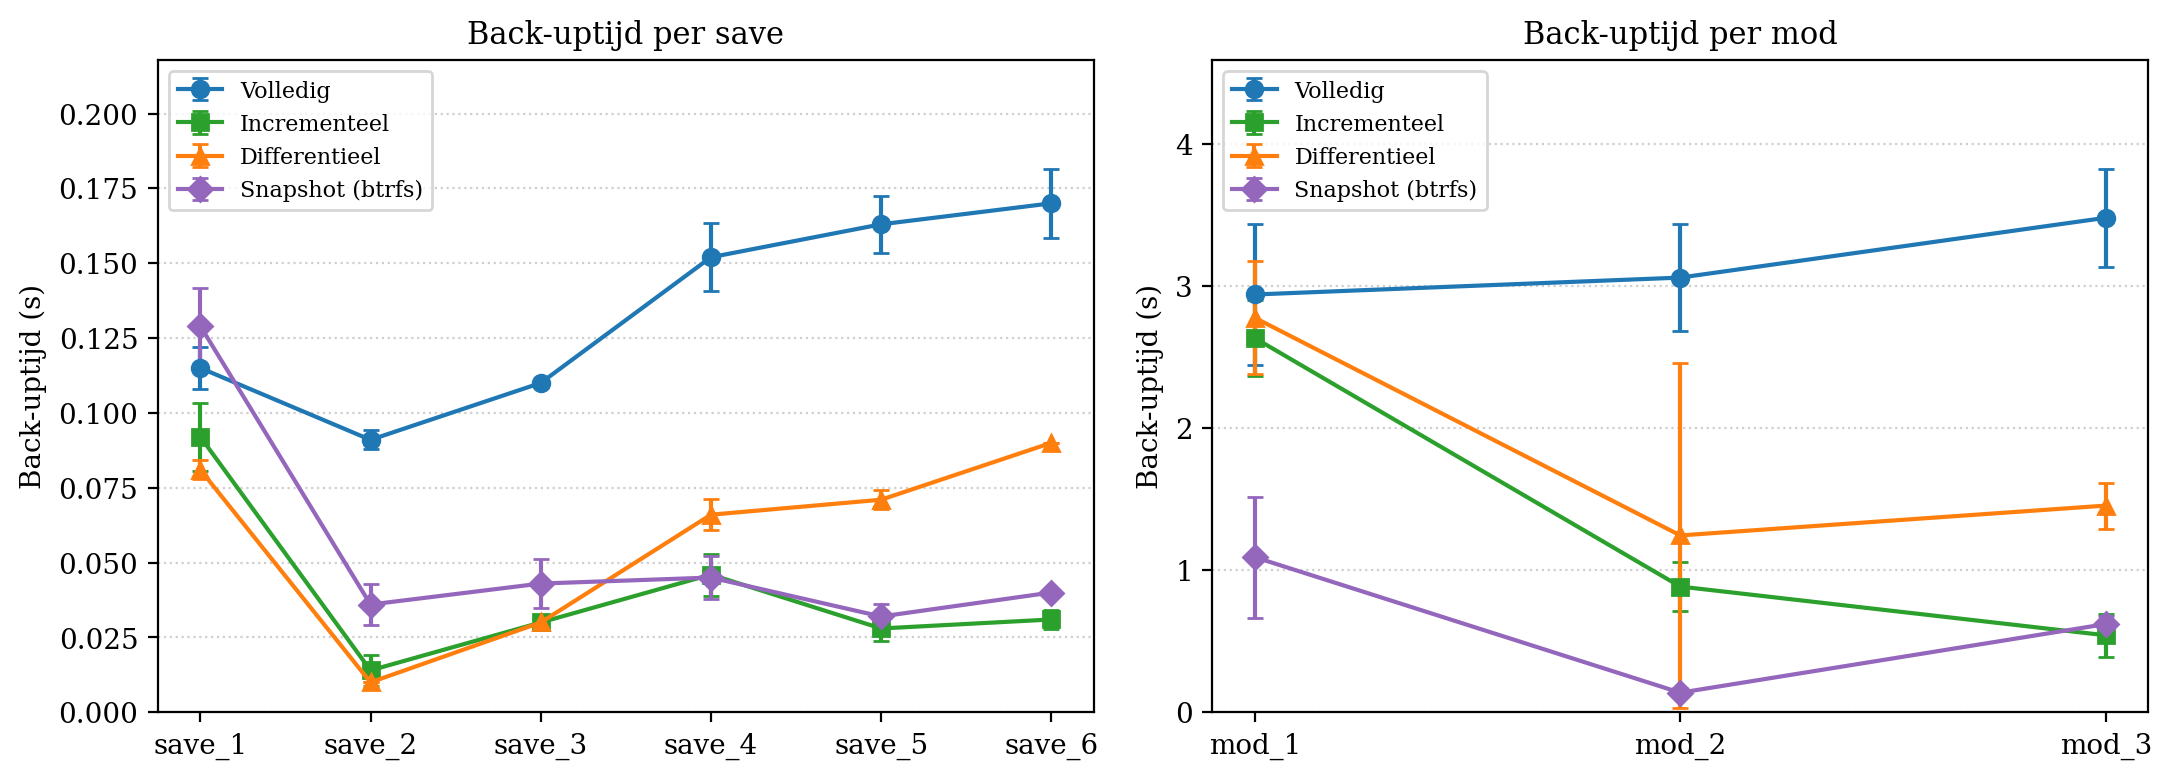
\includegraphics[width=\linewidth]{figures/fig_backup_time_per_point.png}
    \caption{Back-uptijd per individueel back-uppunt (gemiddelde over 10 runs, foutbalken: standaardafwijking). \textbf{Let op:} de y-assen verschillen sterk in schaal omdat de moddataset twee orden van grootte groter is dan de savedataset.}
    \label{fig:backup-time}
\end{figure}

\paragraph{Volledige back-up.}
Bij beide datasets stijgt de back-uptijd voor de volledige methode nagenoeg monotoon met de grootte van de te archiveren folder. Bij de saves stijgt de tijd van $\sim$0{,}11~s voor \texttt{save\_1} tot $\sim$0{,}17~s voor \texttt{save\_6}, in lijn met het feit dat \texttt{save\_6} ongeveer dubbel zo groot is als \texttt{save\_1}. Bij de mods volgt de tijd dezelfde tendens ($\sim$2{,}94~s voor \texttt{mod\_1} tot $\sim$3{,}48~s voor \texttt{mod\_3}). Het belangrijke inzicht is dat de tijd bij de volledige methode niet afhankelijk is van eerdere back-uppunten: elke back-up is een onafhankelijke, volledige kopie en de kost wordt enkel bepaald door de huidige grootte.

\paragraph{Incrementele back-up.}
Bij de saves toont de incrementele methode het meest karakteristieke gedrag. \texttt{save\_1} kost $\sim$0{,}09~s — vrijwel identiek aan de volledige back-up van diezelfde save, want het is per definitie hetzelfde volledige basisarchief. \texttt{save\_2} valt vervolgens terug naar slechts $\sim$0{,}014~s, zes keer sneller dan \texttt{save\_1}. Dit geeft de kerneigenschap van de incrementele strategie weer: \texttt{save\_2} verschilt zeer weinig van \texttt{save\_1} en het increment bevat dus nauwelijks data. Vanaf \texttt{save\_3} schommelt de tijd tussen $\sim$0{,}03~s en $\sim$0{,}05~s, afhankelijk van het volume aan tussentijdse wijzigingen. \texttt{save\_4} ligt duidelijk hoger dan de andere savepunten, wat overeen komt met een groter increment-archief op datzelfde punt (zie verder, sectie~\ref{subsec:storage}). Bij de mods is hetzelfde patroon zichtbaar: \texttt{mod\_1} duurt $\sim$2{,}63~s als basisarchief, \texttt{mod\_2} valt terug naar $\sim$0{,}88~s en \texttt{mod\_3} naar slechts $\sim$0{,}54~s.

\paragraph{Differentiële back-up.}
Voor de differentiële methode is \texttt{save\_2} (en \texttt{mod\_2}) even goedkoop als bij de incrementele methode. Er is op dat moment nog geen verschil tussen ``ten opzichte van de basis'' en ``ten opzichte van de vorige''. Vanaf het derde back-uppunt divergeren de twee methodes wel. Bij de saves stijgt de differentiële back-uptijd van $\sim$0{,}03~s (\texttt{save\_3}) tot $\sim$0{,}09~s (\texttt{save\_6}), terwijl de incrementele tijd in dezelfde range schommelt rond $\sim$0{,}03~s. Bij de mods is het verschil duidelijker: \texttt{mod\_3} kost $\sim$1{,}45~s differentieel tegenover $\sim$0{,}54~s incrementeel. Dit komt doordat de differentiële methode telkens alle wijzigingen ten opzichte van de basis-back-up moet meenemen, waardoor de archieven cumulatief groeien naarmate er meer back-ups worden gemaakt.

\paragraph{Snapshot.}
De snapshotmethode vertoont een fundamenteel ander gedrag. Bij de saves kost de eerste snapshot ($\sim$0{,}13~s) iets meer dan de daarop volgende ($\sim$0{,}03 -- 0{,}05~s). Dit is vermoedelijk te wijten aan het initialiseren van quota-administratie van het bestandssysteem. Vanaf \texttt{save\_2} is de tijd nagenoeg constant en grotendeels onafhankelijk van de grootte van de save. Bij de mods is hetzelfde patroon zichtbaar, met opmerkelijke uitschieters: \texttt{mod\_2} wordt in $\sim$0{,}14~s gesnapshot, acht keer sneller dan \texttt{mod\_1}. Deze uitschieter is mogelijk te wijten aan I/O-caching tussen opeenvolgende runs (de blokken van \texttt{mod\_2} bevinden zich nog in het page cache na de back-up van \texttt{mod\_1}). De brede foutbalk bij \texttt{mod\_1} bevestigt dat de eerste snapshot in een sessie meer variabiliteit vertoont. Wat wel consistent is, is dat de snapshotmethode in geen enkel geval afhangt van het cumulatieve werk van eerdere back-uppunten.

\subsection{CPU-gebruik tijdens de back-up}
\label{subsec:backup-cpu}

Figuur~\ref{fig:backup-cpu} toont het CPU-gebruik per back-uppunt.

\begin{figure}[h]
    \centering
    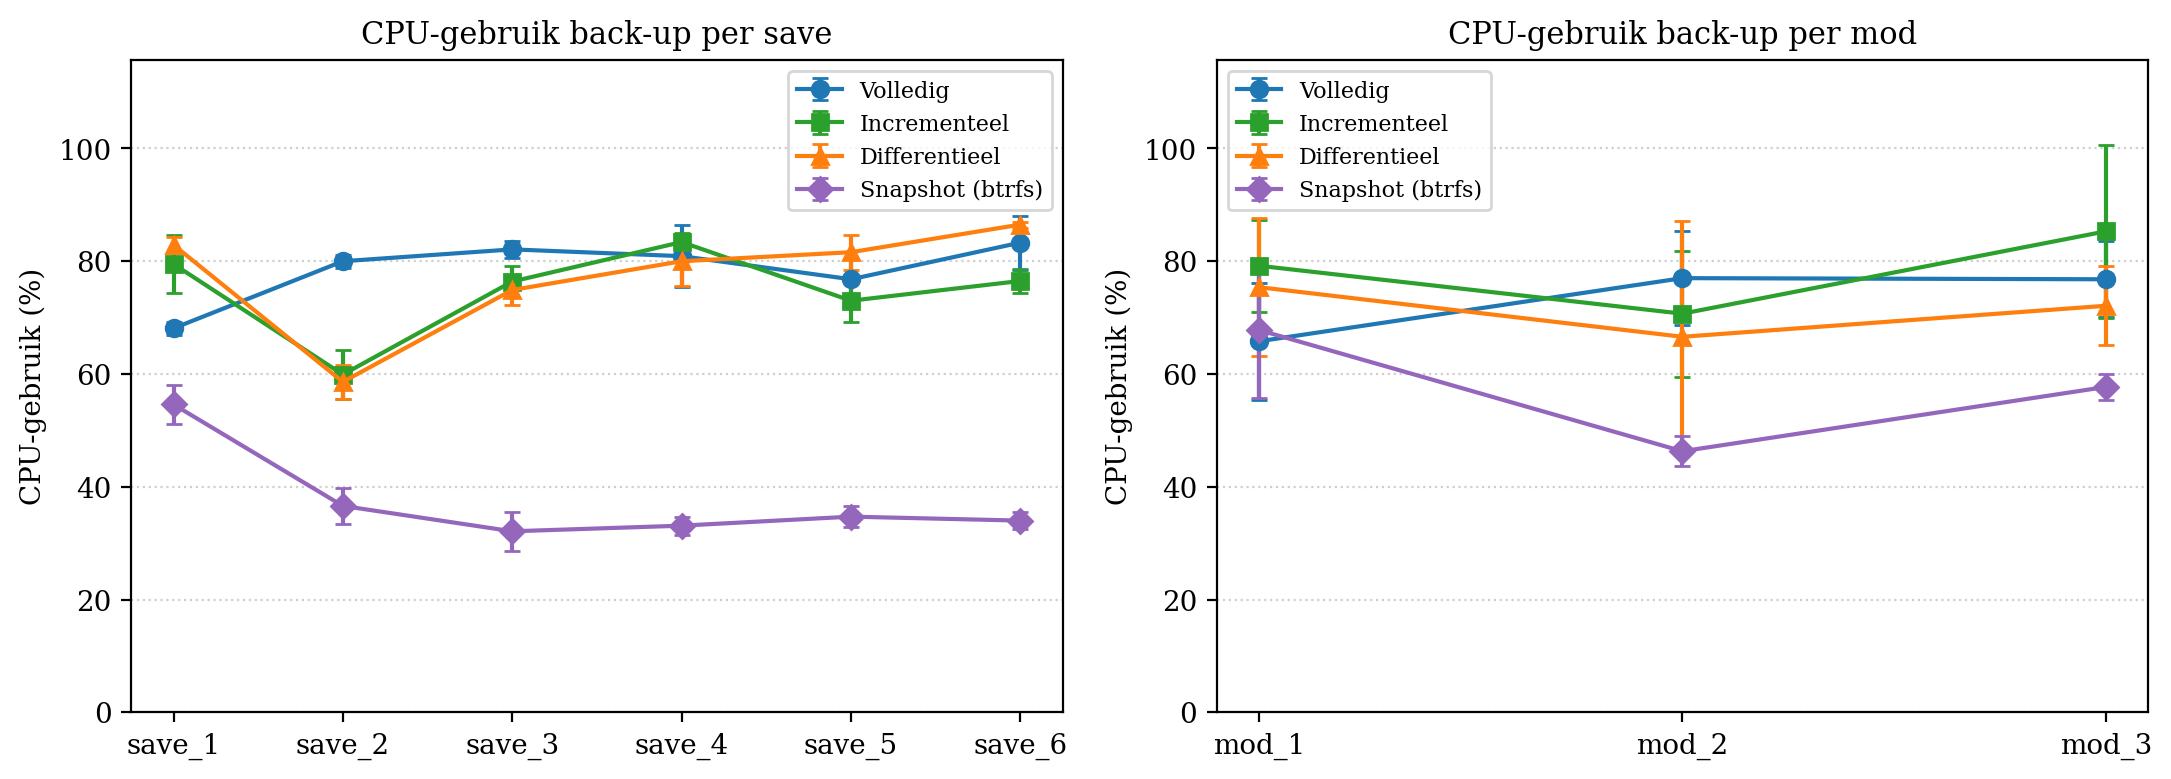
\includegraphics[width=\linewidth]{figures/fig_backup_cpu_per_point.png}
    \caption{CPU-gebruik tijdens de back-upfase, per individueel back-uppunt. De y-as is voor beide grafieken gelijkgeschaald. Een waarde van 100\% komt overeen met één volledige thread; het maximum op deze 16-thread-CPU is 1600\%.}
    \label{fig:backup-cpu}
\end{figure}

Voor de tar-gebaseerde methodes ligt het CPU-gebruik consistent tussen $\sim$60\% en $\sim$85\%. Bij de saves valt op dat \texttt{save\_2} bij zowel incrementeel als differentieel een lager CPU-gebruik toont ($\sim$60\%). Wanneer het increment zeer klein is en de operatie slechts $\sim$10~ms duurt, domineert de opstartoverhead van \texttt{tar} en hoeft de eigenlijke verwerking nauwelijks rekenwerk. Voor de mods, waar elke operatie ten minste een halve seconde duurt, ligt de CPU-utilisatie stabieler tussen 65\% en 85\%.

De snapshotmethode toont een lager CPU-gebruik (25--70\%). Het aanmaken van een btrfs-snapshot is grotendeels een metadata-operatie die in de kernel wordt afgehandeld, het user-space proces (\texttt{btrfs subvolume snapshot}) is zeer kort actief.

\subsection{Geheugengebruik}
\label{subsec:backup-mem}

Figuur~\ref{fig:backup-mem} toont het piek-RSS per back-uppunt.

\begin{figure}[h]
    \centering
    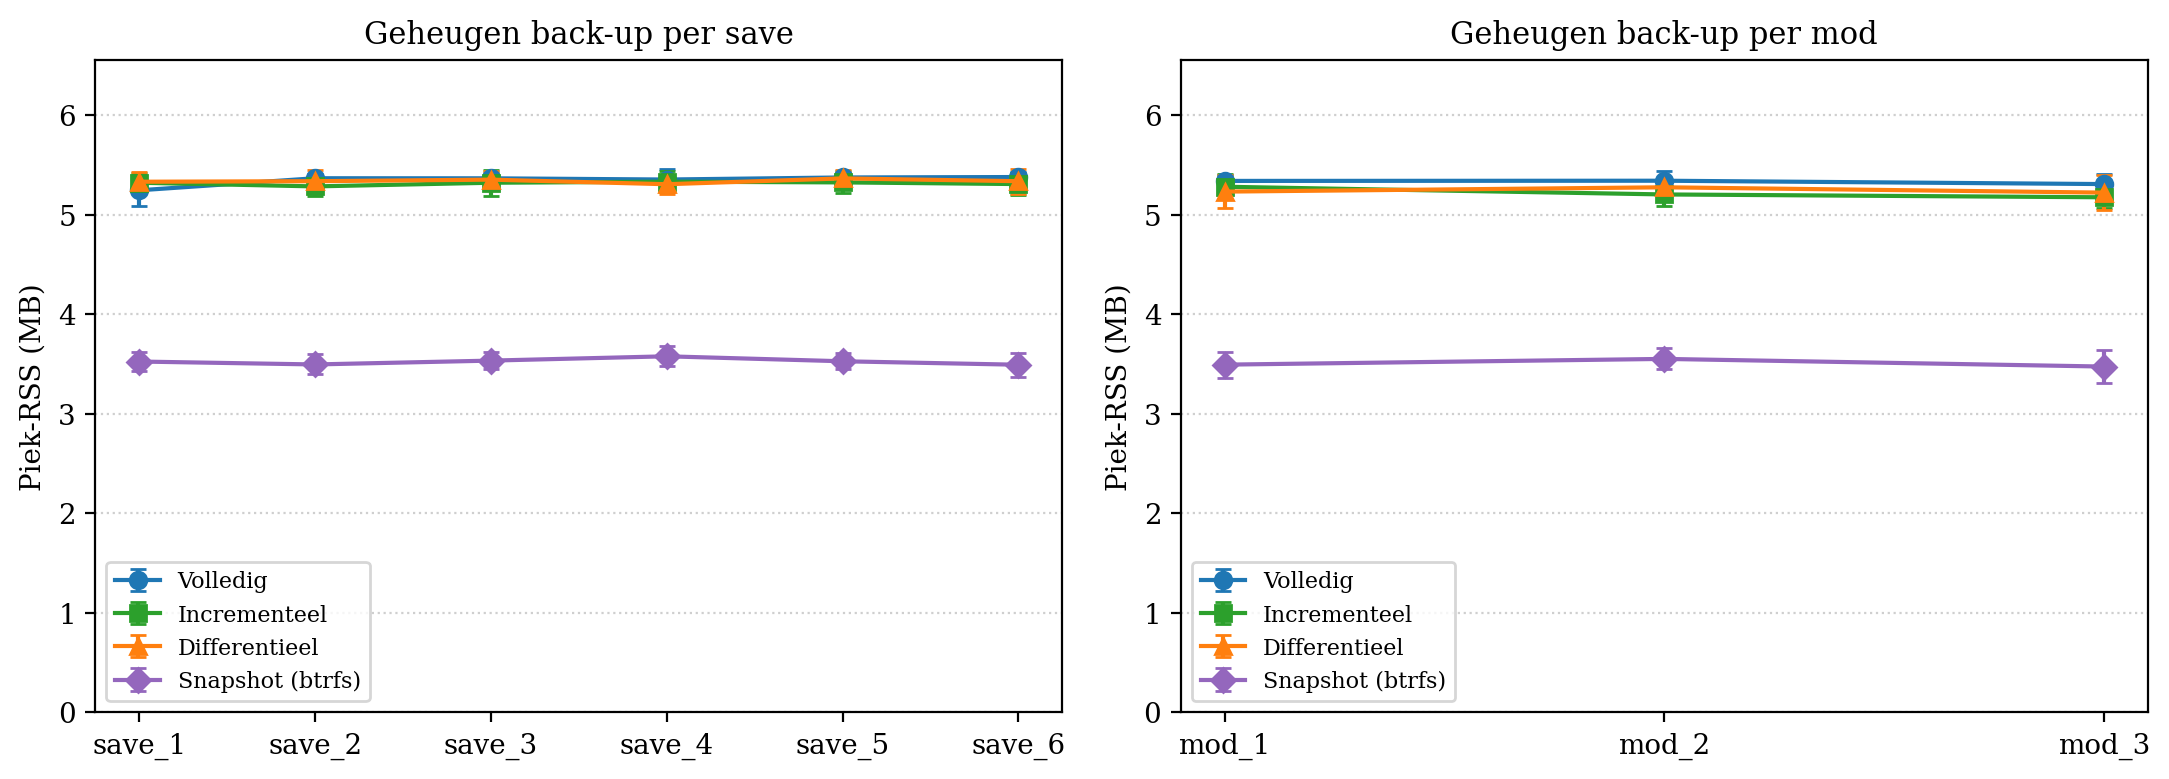
\includegraphics[width=\linewidth]{figures/fig_backup_mem_per_point.png}
    \caption{Piek-RSS van het back-upproces, per individueel back-uppunt. De y-as is identiek geschaald voor beide datasets.}
    \label{fig:backup-mem}
\end{figure}

Het geheugengebruik blijkt onafhankelijk van zowel de methode als de grootte van het te archiveren item. Alle tar-runs liggen tussen 5{,}3 en 5{,}5~MB; de snapshot-runs liggen telkens rond de 3{,}6~MB. \texttt{tar} streamt de invoer en houdt geen volledig archief in het geheugen, waardoor het geheugengebruik niet verschilt op basis van de archief grootte. Op moderne systemen vormt geheugen geen bottleneck voor deze werklast. Wat wel opvalt is dat het geheugengebruik van de snapshotmethode een stuk lager ligt. Dit toont nog eens aan hoe weinig werk een snapshot nemen inhoudt.

\subsection{Opslaggebruik}
\label{subsec:storage}

Figuur~\ref{fig:storage} toont de archiefgrootte per back-uppunt voor de drie tar-methodes. Voor de snapshotmethode wordt de opslag apart besproken in figuren~\ref{fig:snapshot-storage-saves} en~\ref{fig:snapshot-storage-mods}, omdat het concept van ``archiefgrootte'' daar niet van toepassing is.

\begin{figure}[h]
    \centering
    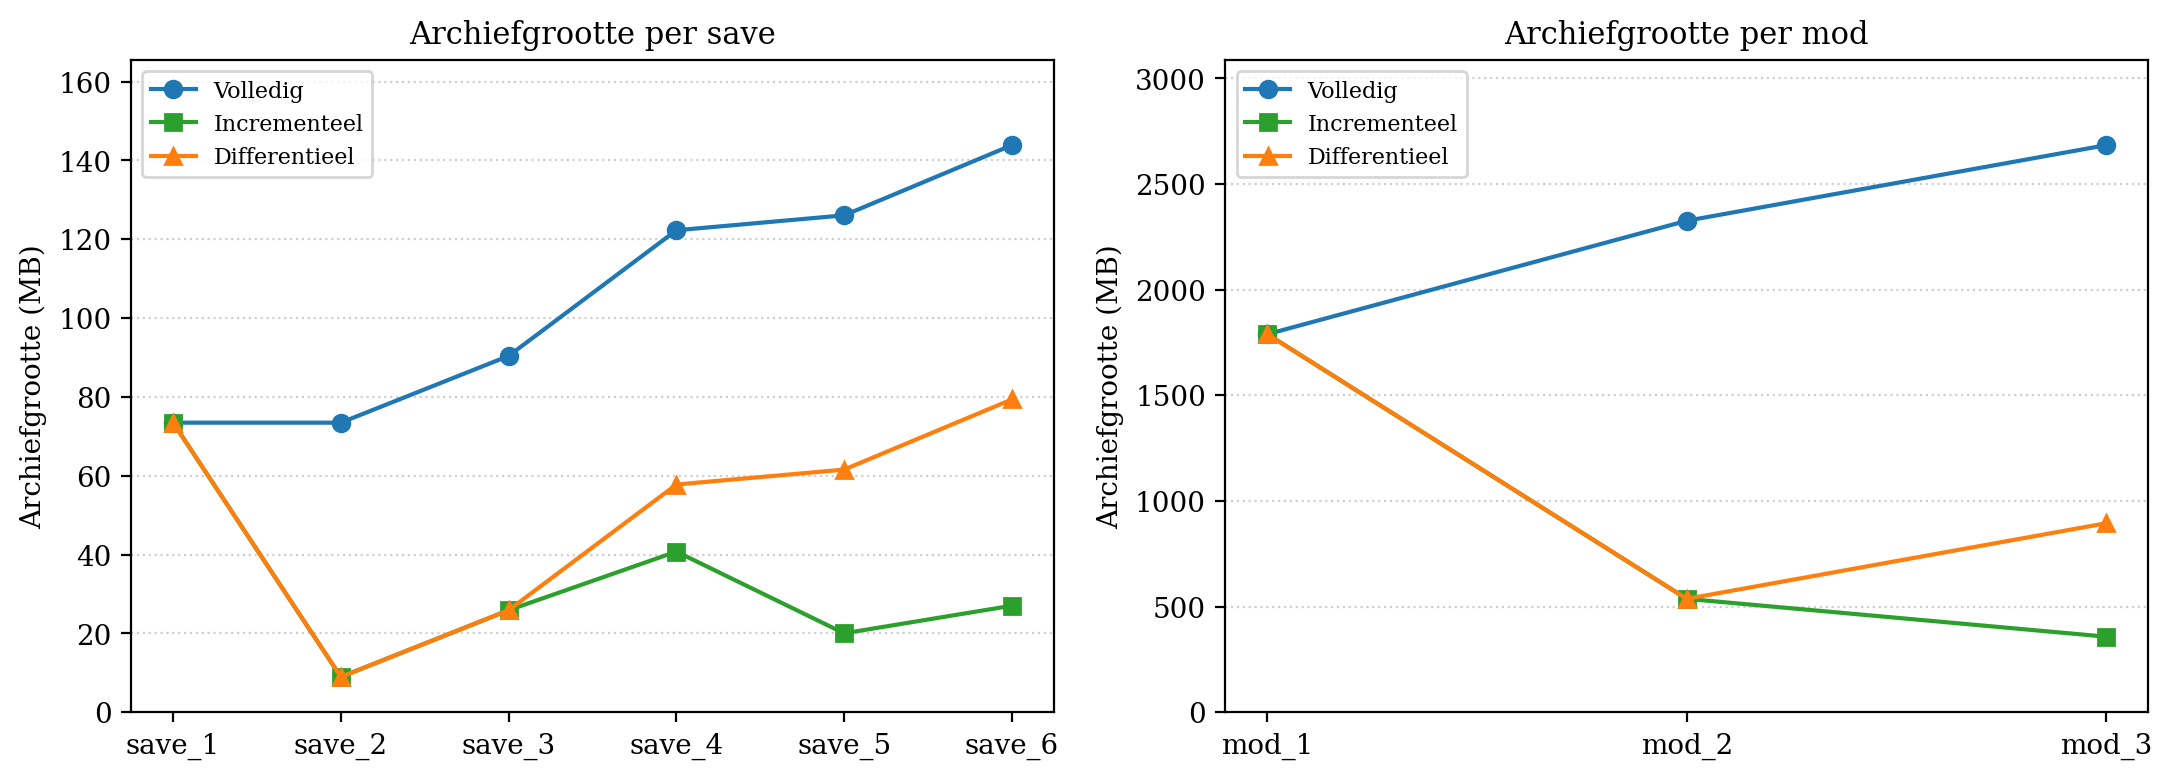
\includegraphics[width=\linewidth]{figures/fig_storage_per_point.png}
    \caption{Archiefgrootte per individueel back-uppunt voor de tar-gebaseerde methodes.}
    \label{fig:storage}
\end{figure}

\paragraph{Volledige back-up.}
Bij de saves stijgt de archiefgrootte van $\sim$73~MB (\texttt{save\_1}) tot $\sim$144~MB (\texttt{save\_6}) en bij de mods van $\sim$1{,}79~GB (\texttt{mod\_1}) tot $\sim$2{,}68~GB (\texttt{mod\_3}). Elke back-up bevat de volledige actuele broninhoud, zonder enige optimalisatie tussen back-uppunten. De cumulatieve opslaggrootte is dus gelijk aan de som van alle balken: ongeveer 630~MB voor de zes saves en 6{,}80~GB voor de drie mods.

\paragraph{Incrementele back-up.}
De grafiek toont het kenmerkende patroon van de incrementele methode. \texttt{save\_1} (en \texttt{mod\_1}) is volledig en daardoor identiek in grootte aan de volledige back-up. \texttt{save\_2} valt terug naar slechts $\sim$9~MB. Daarna fluctueert de archiefgrootte met de hoeveelheid tussentijdse wijzigingen: \texttt{save\_4} geeft een piek ($\sim$41~MB), wat correspondeert met een grotere speelsessie met meer wijzigingen. Bij de mods levert \texttt{mod\_2} een increment van $\sim$537~MB en \texttt{mod\_3} slechts $\sim$358~MB op: de update naar mod-versie 3 bevat dus minder gewijzigde data dan de update naar versie 2. De cumulatieve opslagvoetafdruk komt op $\sim$196~MB voor de saves (een besparing van 69\% ten opzichte van de volledige methode) en $\sim$2{,}68~GB voor de mods (besparing van 60\%).

\paragraph{Differentiële back-up.}
Het verschil met incrementeel wordt onmiddellijk duidelijk. Voor \texttt{save\_2} en \texttt{mod\_2} is de archiefgrootte identiek aan de incrementele variant, omdat het differentieel op dat moment gelijk is aan het increment. Vanaf het derde back-uppunt divergeert differentieel: \texttt{save\_4} is $\sim$58~MB tegenover $\sim$41~MB incrementeel, en \texttt{save\_6} is $\sim$79~MB tegenover $\sim$27~MB incrementeel. Bij de mods is \texttt{mod\_3} zelfs $\sim$895~MB tegenover $\sim$358~MB incrementeel, een verschil van bijna 540~MB voor hetzelfde back-uppunt. Cumulatief loopt dit op tot $\sim$307~MB voor de saves en $\sim$3{,}22~GB voor de mods.

\paragraph{Snapshot.}
Voor de snapshotmethode wordt de opslag op twee manieren weergegeven in figuren~\ref{fig:snapshot-storage-saves} en~\ref{fig:snapshot-storage-mods}: enerzijds de marginale kost per individuele snapshot (de exclusieve datagrootte), anderzijds de cumulatieve fysieke voetafdruk van de hele snapshot-set naarmate er meer back-uppunten worden toegevoegd.

\begin{figure}[h]
    \centering
    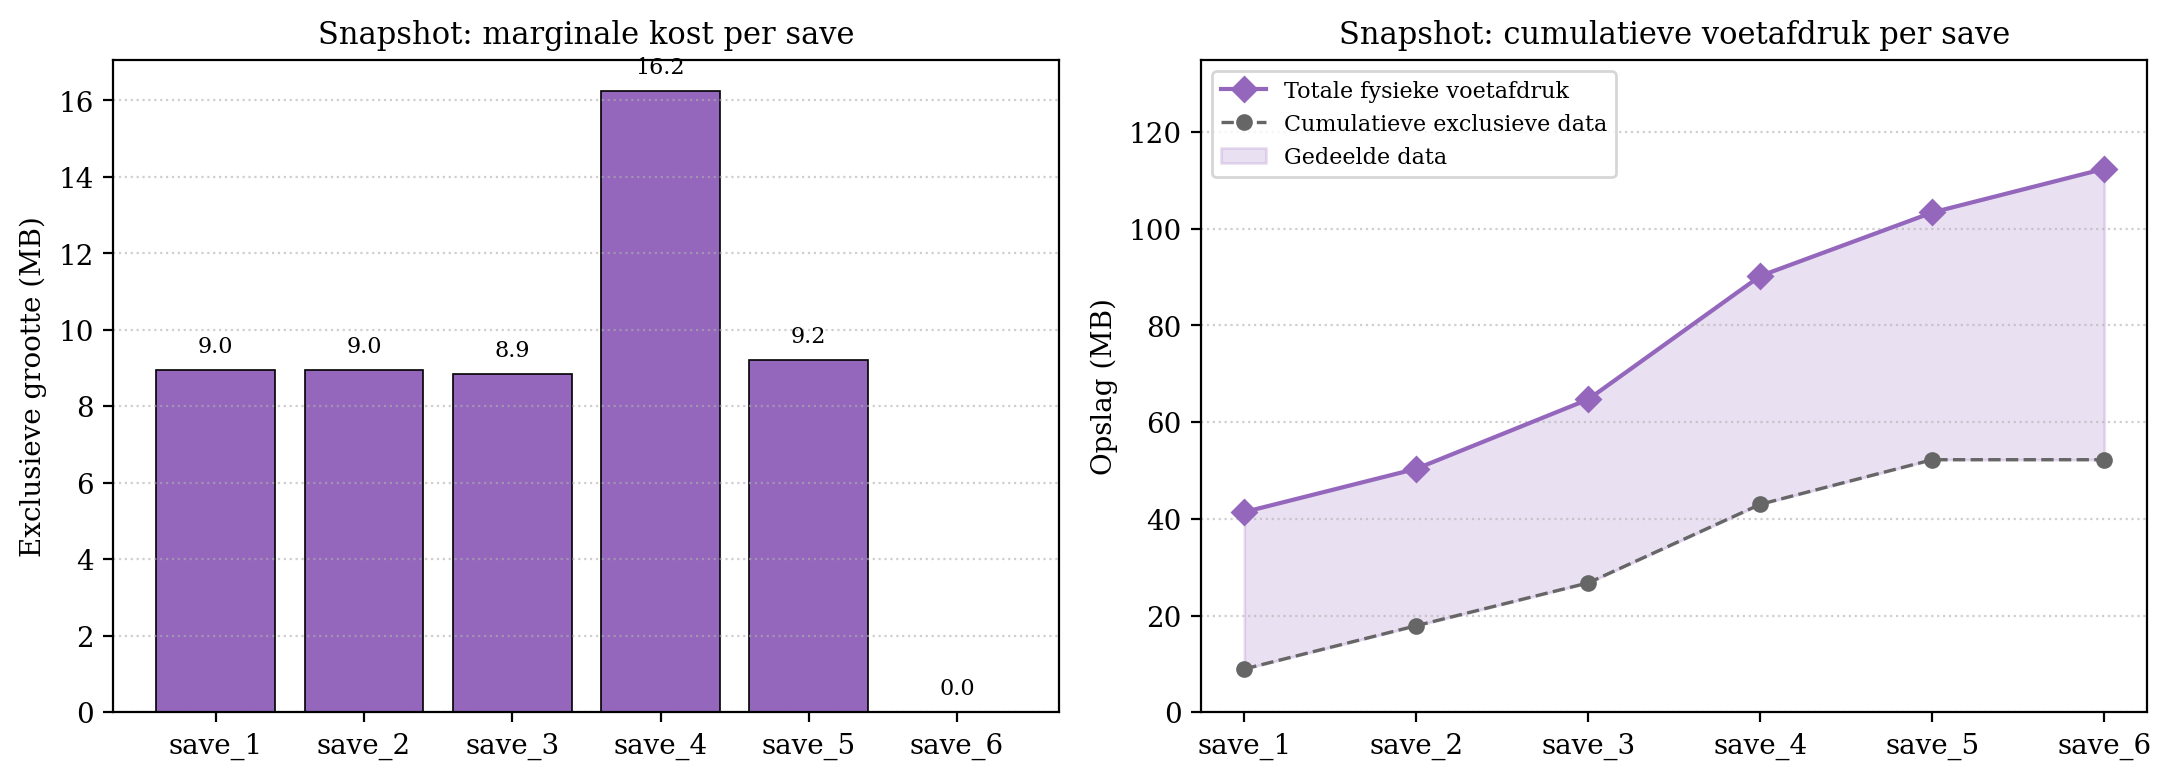
\includegraphics[width=\linewidth]{figures/fig_snapshot_storage_saves.png}
    \caption{Opslagprofiel van de snapshotmethode voor de saves. Links: de marginale kost per snapshot (exclusieve data, dus blokken die niet door andere snapshots of het bronvolume worden gedeeld). Rechts: de totale fysieke voetafdruk van de snapshot-set, opgesplitst in cumulatieve exclusieve data (onderaan) en gedeelde data (gevulde zone).}
    \label{fig:snapshot-storage-saves}
\end{figure}

\begin{figure}[h]
    \centering
    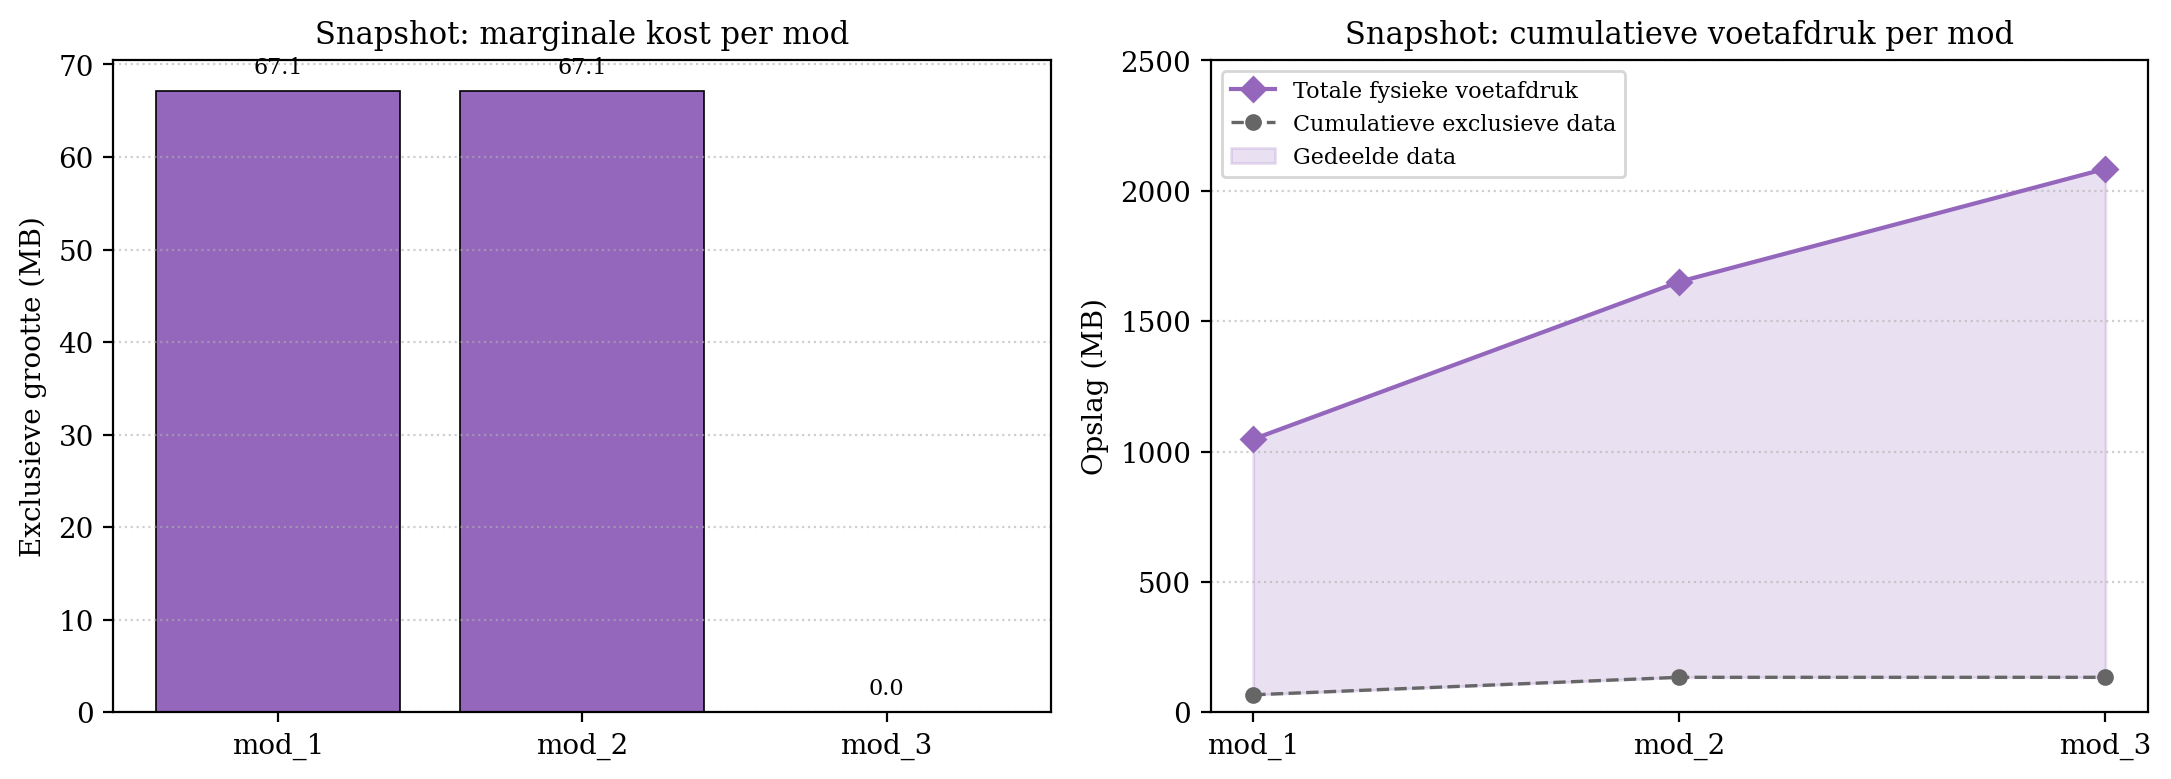
\includegraphics[width=\linewidth]{figures/fig_snapshot_storage_mods.png}
    \caption{Opslagprofiel van de snapshotmethode voor de mods. Zelfde structuur als figuur~\ref{fig:snapshot-storage-saves}.}
    \label{fig:snapshot-storage-mods}
\end{figure}

Bij de saves is de marginale kost per snapshot zeer uniform: elk van de eerste vijf snapshots draagt ongeveer 9~MB aan exclusieve data bij, met één duidelijke uitschieter (\texttt{save\_4}: 16~MB). Deze uitschieter komt opnieuw overeen met de hoger genoemde gameplay-piek tussen \texttt{save\_3} en \texttt{save\_4}: meer gewijzigde blokken impliceert meer data die exclusief in de voorafgaande snapshot achterblijft wanneer het bronvolume verandert. \texttt{save\_6} heeft een exclusieve grootte van 0~MB; dit punt representeert de actuele toestand van het bronvolume, waardoor al zijn blokken nog gedeeld zijn. De cumulatieve voetafdruk groeit lineair van $\sim$41~MB (één snapshot) tot $\sim$112~MB (zes snapshots), een fractie van de 196~MB die de incrementele strategie nodig heeft voor dezelfde back-ups.

Bij de mods is het beeld vergelijkbaar: zowel \texttt{mod\_1} als \texttt{mod\_2} bevatten elk $\sim$67~MB exclusieve data, terwijl \texttt{mod\_3} (de actuele broninhoud) 0~MB exclusief heeft. De cumulatieve voetafdruk bedraagt $\sim$2{,}07~GB voor de drie mod-snapshots, tegenover $\sim$2{,}68~GB voor de incrementele tar-strategie en $\sim$6{,}80~GB voor de volledige tar-strategie.

Een belangrijke nuance is dat de ratio tussen exclusieve en gedeelde data afhangt van hoeveel het bronvolume tussen back-uppunten wijzigt. Een mod-update die volledig nieuwe assets installeert, verschuift al die nieuwe blokken van ``gedeeld'' naar ``exclusief'' aan de oude snapshot. In het slechtste geval, waarbij elke snapshot volledig divergeert van de volgende, verzwakt de snapshotmethode qua opslagverbruik tot in de buurt van volledige back-ups. In de praktijk is dit zeldzaam voor mods en savegames, waar de overgrote meerderheid van de blokken intact blijft tussen opeenvolgende back-uppunten.


\section{Resultaten: restorefase}
\label{sec:results-restore}

Het herstellen van een back-up is voor de eindgebruiker minstens even belangrijk als de back-up zelf: een rollback wordt vrijwel altijd uitgevoerd in een situatie van tijdsdruk (een mod heeft de installatie gebroken, een savegame is corrupt). De restoretijd bepaalt hoe lang de gebruiker moet wachten om opnieuw te kunnen spelen. Zoals toegelicht in~\ref{subsec:meetvelden} is de gerapporteerde restoretijd voor incrementele en differentiële methodes \emph{cumulatief}: de tijd die nodig is om alle archieven uit te pakken die nodig zijn om het gewenste back-uppunt te herstellen.

\subsection{Snelheid van de restore}
\label{subsec:restore-time}

Figuur~\ref{fig:restore-time} toont de restoretijd per back-uppunt.

\begin{figure}[h]
    \centering
    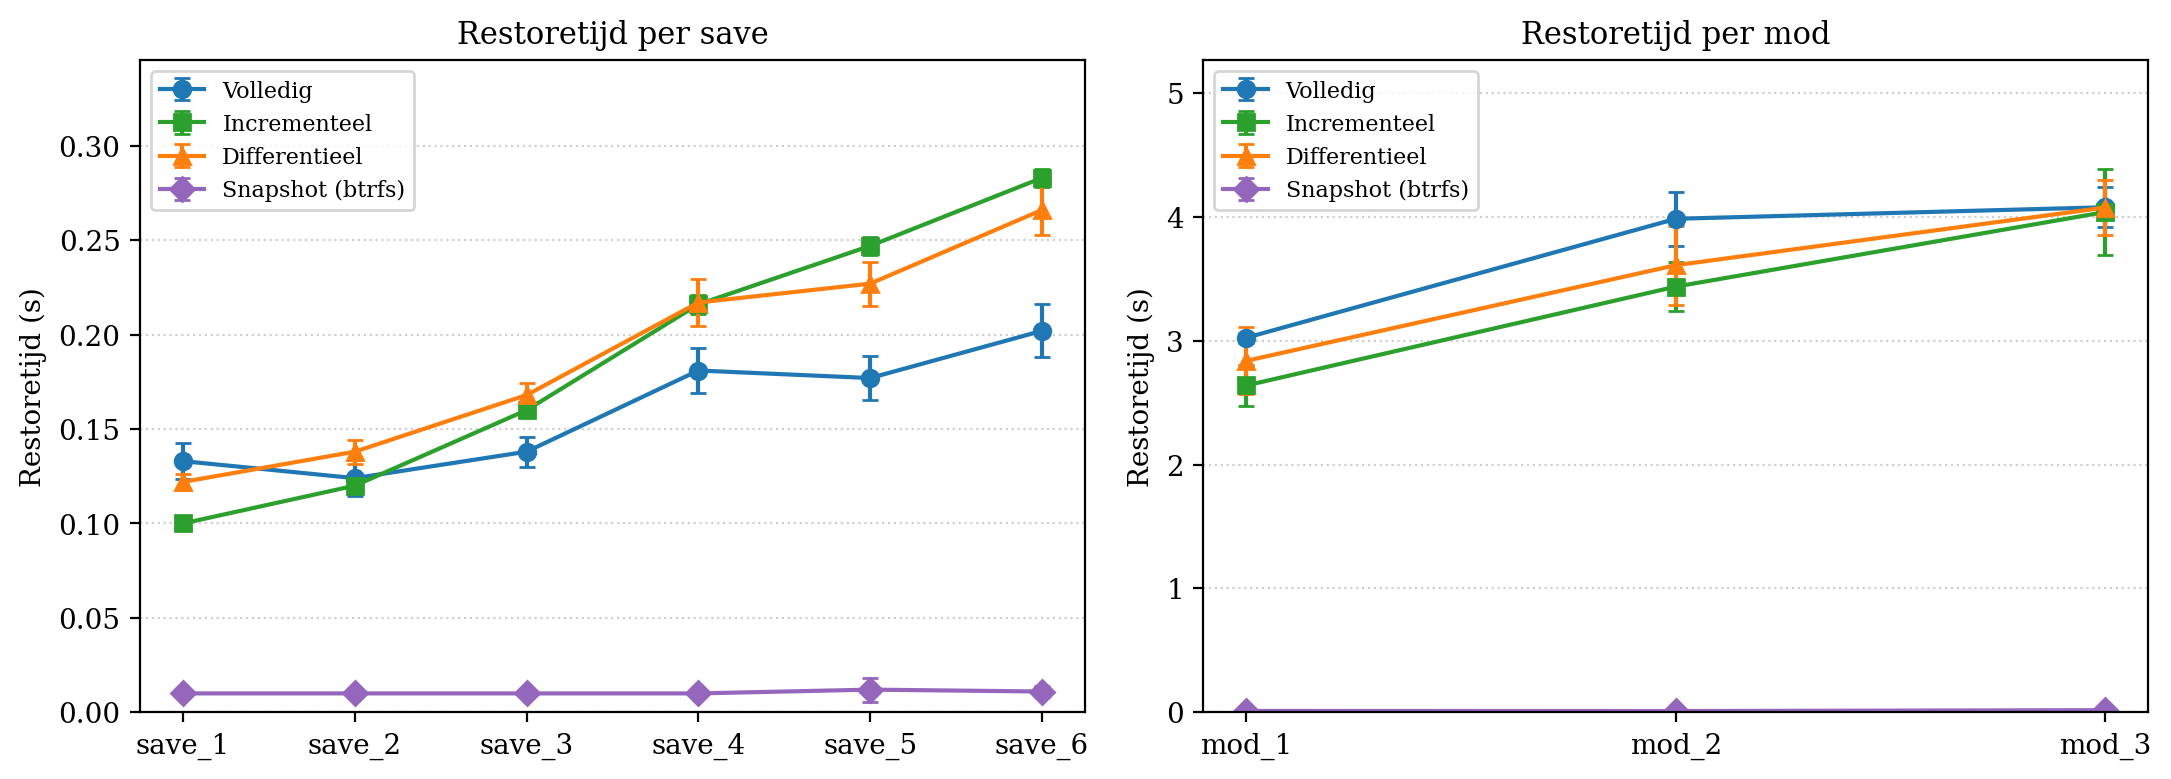
\includegraphics[width=\linewidth]{figures/fig_restore_time_per_point.png}
    \caption{Restoretijd per back-uppunt. De gerapporteerde tijd is de cumulatieve duur om alle archieven uit te pakken die nodig zijn om dat back-uppunt te herstellen.}
    \label{fig:restore-time}
\end{figure}

\paragraph{Volledige restore.}
Bij de saves stijgt de restoretijd geleidelijk van $\sim$0{,}13~s (\texttt{save\_1}) tot $\sim$0{,}20~s (\texttt{save\_6}), dit komt overeen met de groei van de archiefgrootte. Bij de mods zijn de restoretijden zeer gelijkaardig onder de verschillende methodes. Met \texttt{mod\_2} een verwaarloosbaar stuk langer dan incrementeel en differentieel rond $\sim$3{,}96~s.

\paragraph{Incrementele restore.}
De restoretijd stijgt zeer gelijmatig met elk back-uppunt, zowel bij saves ($\sim$0{,}10~s voor \texttt{save\_1} tot $\sim$0{,}28~s voor \texttt{save\_6}) als bij mods ($\sim$2{,}64~s voor \texttt{mod\_1} tot $\sim$4{,}04~s voor \texttt{mod\_3}). Dit lineaire verband is een direct gevolg van de cumulatieve aard van een incrementele restore: om \texttt{save\_6} terug te zetten moeten zes archieven sequentieel worden uitgepakt (basis + vijf incrementen), elk met zijn eigen overhead. Bij latere back-uppunten loopt deze opstartoverhead op en wordt de incrementele restore zelfs trager dan een volledige restore vanaf hetzelfde punt, bij de saves is dit duidelijk vanaf \texttt{save\_3}.

\paragraph{Differentiële restore.}
Differentieel bevindt zich tussen volledig en incrementeel. Het restoreproces vereist altijd exact twee archieven: de basis-back-up en de differentiële back-up van het gewenste punt. Daardoor is de opstartoverhead constant, maar de hoeveelheid uit te pakken data groeit mee met de grootte van het differentieel-archief. Voor de saves gedraagt de differentiële restore zich vrijwel identiek aan de incrementele ($\sim$0{,}12~s tot $\sim$0{,}27~s). bij de mods ligt \texttt{mod\_2} bij $\sim$3{,}61~s en \texttt{mod\_3} bij $\sim$4{,}07~s, ook gelijk aan incrementeel.

\paragraph{Snapshot-restore.}
Een snapshot-restore vergt in alle geteste configuraties slechts $\sim$10--17~ms, ongeacht de back-up. De operatie bestaat in essentie uit het hernoemen of swappen van het subvolume. Er moet dus geen data verplaatst worden. In een rollbackscenario is dit een groot verschil tegenover de tar-methodes: voor een mod-rollback is \texttt{btrfs} hier ruim 200 keer sneller dan de snelste tar-methode.

\subsection{CPU-gebruik tijdens de restore}
\label{subsec:restore-cpu}

Figuur~\ref{fig:restore-cpu} toont het CPU-gebruik per back-uppunt tijdens de restorefase.

\begin{figure}[h]
    \centering
    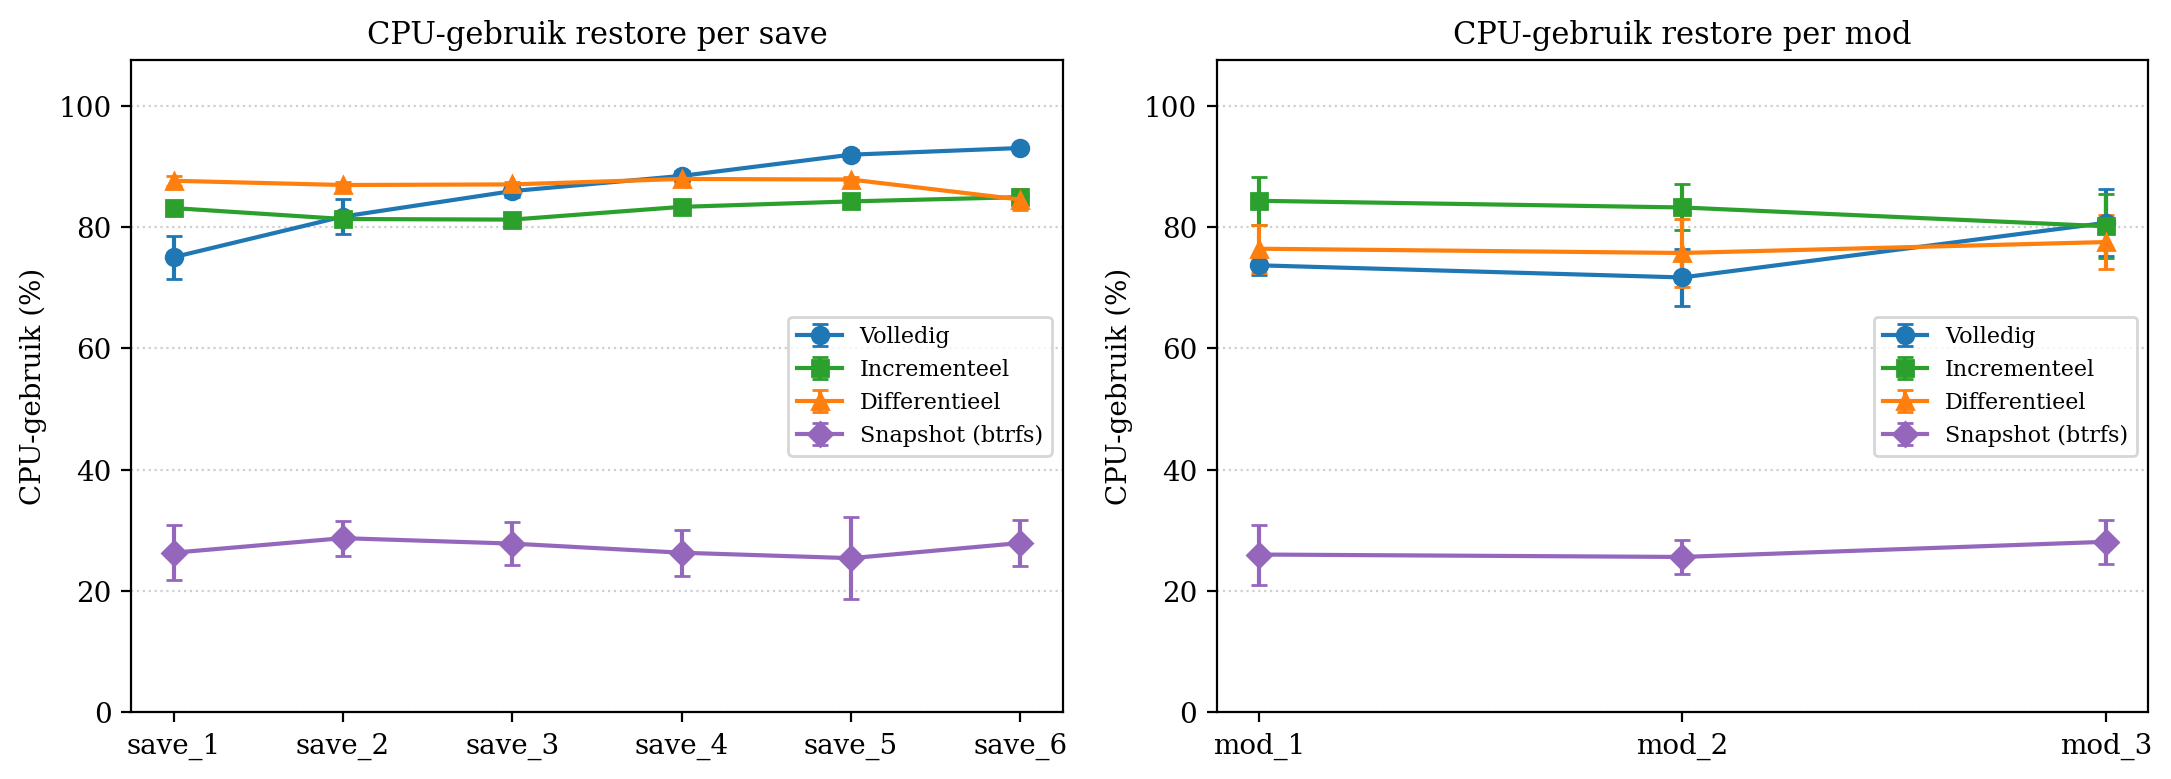
\includegraphics[width=\linewidth]{figures/fig_restore_cpu_per_point.png}
    \caption{CPU-gebruik tijdens de restorefase, per back-uppunt. De y-as is voor beide grafieken gelijk.}
    \label{fig:restore-cpu}
\end{figure}

Voor de tar-gebaseerde methodes ligt het CPU-gebruik tussen 75\% en 93\%, met de saves consistent hoger dan de mods. Dit toont aan dat het uitpakken van veel kleine bestanden CPU-intensiever is dan het uitpakken van weinig grote bestanden, wat overeenstemt met het idee dat de overhead per bestand (metadata-aanmaak, attribuut-toewijzing) zwaarder weegt naarmate er meer bestanden zijn. Bij de volledige restore van de saves stijgt het CPU-gebruik licht met elke back-up (van 75\% bij \texttt{save\_1} tot 93\% bij \texttt{save\_6}), wat overeenkomt met de groei van het archief en de toename van het aantal te schrijven bestanden.

De snapshot-restore blijft, net als bij de back-up, op $\sim$25--28\% en illustreert opnieuw dat het hier in gewoon om een metadata-operatie gaat.


\section{Synthese en conclusie}
\label{sec:synthese}

\subsection{Samenvattende vergelijking}

Tabel~\ref{tab:summary} vat de belangrijkste meetwaarden samen, geaggregeerd over alle back-uppunten heen om een overzichtelijke totaalbeeld te geven. De cijfers in deze tabel zijn sommen over de volledige dataset (de zes saves of de drie mods).

\begin{table}[h]
    \centering
    \caption{Samenvattende vergelijking van back-upmethodes zonder compressie, geaggregeerd over de hele dataset. Tijden in seconden, opslag in MB}
    \label{tab:summary}
    \small
    \begin{tabular}{lrrrrrr}
        \toprule
        & \multicolumn{3}{c}{\textbf{Saves (6 stuks, $\sim$0{,}6~GB)}}
        & \multicolumn{3}{c}{\textbf{Mods (3 stuks, $\sim$6{,}5~GB)}} \\
        \cmidrule(lr){2-4}\cmidrule(lr){5-7}
        \textbf{Methode} & Back-up & Restore & Opslag
        & Back-up & Restore & Opslag \\
        \midrule
        Volledig       & 0{,}80 & 0{,}96 &  630 &  9{,}48 & 11{,}05 & 6800 \\
        Incrementeel   & 0{,}24 & 1{,}13 &  196 &  4{,}06 & 10{,}11 & 2684 \\
        Differentieel  & 0{,}35 & 1{,}14 &  307 &  5{,}48 & 10{,}52 & 3221 \\
        Snapshot       & 0{,}33 & 0{,}06 &  112$^{\ast}$ & 1{,}85 & 0{,}04  & 2070$^{\ast}$ \\
        \bottomrule
    \end{tabular}
    
    \vspace{0.4em}
    \footnotesize $^{\ast}$ Voor de snapshotmethode betreft de vermelde opslag de \emph{totale fysieke voetafdruk} van de volledige snapshot-set, inclusief de gedeelde blokken die fysiek slechts één keer worden bewaard.
\end{table}

\subsection{Per-back-up observaties}

De analyse per back-uppunt brengt een aantal patronen aan het licht die in een gesommeerde voorstelling onzichtbaar zouden blijven:

\begin{itemize}
    \item \textbf{Het ``gratis'' tweede back-uppunt bij incrementeel.} Bij zowel saves als mods is het tweede back-uppunt extreem goedkoop in zowel tijd als opslag (\texttt{save\_2}: $\sim$14~ms en 9~MB; \texttt{mod\_2}: $\sim$0{,}88~s en 537~MB). Voor scenario's waarin een gebruiker zeer frequent kleine wijzigingen wenst vast te leggen, levert de incrementele methode een zeer gunstige verhouding op tussen werk en opslagvoetafdruk.
    \item \textbf{Cumulatieve groei van differentiële archieven.} Het verschil tussen incrementeel en differentieel komt pas vanaf het derde back-uppunt aan het licht en groeit daarna geleidelijk. \texttt{mod\_3} differentieel is bijvoorbeeld 2{,}5 keer zo groot als het corresponderende increment. Voor lange reeksen back-uppunten weegt deze cumulatieve groei zwaar door op de totale opslagkost.
    \item \textbf{Cumulatieve groei van incrementele restoretijd.} Hoewel een incrementele back-up zelf goedkoop is, vereist het herstellen ervan het sequentieel uitpakken van alle voorafgaande archieven. Bij de saves wordt incrementele restore vanaf \texttt{save\_4} zelfs trager dan een volledige restore vanaf hetzelfde punt. Dit is een belangrijke afweging: een incrementele strategie minimaliseert het werk per back-up, ten koste van het werk per restore.
    \item \textbf{Voorspelbaarheid van snapshots.} De snapshotmethode vertoont in alle metrieken een constante kost per back-uppunt. Dit staat in scherp contrast met de tar-methodes, waar de individuele kost sterk varieert afhankelijk van de back-up en de tussentijdse wijzigingen. Voor een back-upsysteem dat geautomatiseerd wordt (bijvoorbeeld bij elke mod-update) is voorspelbare kost een belangrijke eigenschap.
    \item \textbf{Blokniveau-deduplicatie van btrfs.} Voor de drie mods samen bedraagt de fysieke voetafdruk van de snapshot-set $\sim$2{,}07~GB, terwijl de incrementele tar-strategie $\sim$2{,}68~GB nodig heeft. Btrfs slaagt erin op blokniveau efficiënter te dedupliceren dan tar op bestandsniveau, zelfs zonder dat er compressie wordt toegepast. Bij de saves is het verschil nog uitgesprokener ($\sim$112~MB tegenover $\sim$196~MB).
\end{itemize}

\subsection{Aanbeveling voor savegames}

Savegames worden frequent overschreven, zijn relatief klein en moeten snel kunnen worden teruggezet. Op basis van de per-back-up analyse:

\begin{itemize}
    \item Op deze schaal zijn alle back-upmethodes sub-seconde per back-up. De keuze wordt daardoor niet bepaald door de back-upsnelheid alleen.
    \item De restoretijd vertoont \emph{wel} een methode-afhankelijk verschil dat oploopt met de back-uppunten. Voor recente back-uppunten (\texttt{save\_5} of \texttt{save\_6}) is een volledige restore sneller dan een incrementele of differentiële restore. Een snapshot-restore is op alle punten ongeveer twintig keer sneller dan welke tar-methode ook.
    \item Het opslagverbruik is in absolute zin verwaarloosbaar (honderden MB op moderne SSDs). Het kleine opslagvoordeel van incrementeel of snapshot weegt hier niet zwaar door.
\end{itemize}

De snapshotmethode is het aantrekkelijkst voor savegames: de constante back-upkost per punt, quasi-instantane rollbacks en een minimale fysieke voetafdruk dankzij copy-on-write. Het belangrijkste nadeel is de afhankelijkheid van btrfs als bestandssysteem. Voor opstellingen waar btrfs niet beschikbaar is, vormt de \emph{incrementele} methode een goed alternatief: de back-uptijd per punt is laag (vaak onder de 50~ms), het opslaggebruik is het zuinigst, en de oplopende restoretijd blijft binnen aanvaardbare grenzen voor savegames van deze omvang. Een volledige back-upstrategie heeft hier geen functioneel voordeel en kost meer ruimte.

\subsection{Aanbeveling voor grote mods}

Voor grote mods is de keuze duidelijker:

\begin{itemize}
    \item De volledige methode is in alle dimensies inferieur. Elke back-up duurt $\sim$3~s en kost $\sim$2~GB aan opslag, ongeacht hoeveel of hoe weinig de mod tussen versies wijzigt. De methode benut bovendien ook geen enkele optimalisatie.
    \item De incrementele methode profiteert sterk van het feit dat opeenvolgende mod-versies veel data delen. \texttt{mod\_3} wordt incrementeel weggeschreven in $\sim$0{,}54~s en kost slechts $\sim$358~MB. Het nadeel is dat een rollback naar een recent punt het sequentieel uitpakken van alle voorgaande versies vereist, met restoretijden die oplopen tot $\sim$4~s.
    \item De differentiële methode biedt geen voordeel ten opzichte van de incrementele. De back-upsnelheid is slechter (meer data per back-up), het opslaggebruik is hoger, en de restoretijd is vergelijkbaar.
    \item De snapshotmethode is opnieuw superieur. Een back-up van een 2{,}5~GB-mod kost $\sim$0{,}6~s en een rollback gebeurt in minder dan 20~ms. De fysieke opslagvoetafdruk voor de drie mod-versies samen ligt bovendien onder die van de incrementele tar-strategie.
\end{itemize}

Voor mods is de winst van btrfs-snapshots zo groot dat dit als voorkeur\-strategie wordt aangenomen wanneer het bestandssysteem ondersteund is. De snelheid van een snapshot-rollback maakt het bovendien mogelijk om \emph{voor elke mod-update} automatisch een back-up\-punt aan te maken, zonder dat de gebruiker een merkbare vertraging ondervindt. Indien btrfs niet beschikbaar is, vormt een incrementele tar-back-up het beste compromis: de eerste back-up duurt $\sim$2{,}6~s (volledig basisarchief), maar daaropvolgende incrementen zijn aanzienlijk lichter.

\section{Analyse van de compressie-algoritmes}
\label{sec:compressie}

\subsection{Doel en opzet van deze analyse}

In dit deel wordt onderzocht welk compressie-algoritme het meest geschikt is om gecombineerd te worden met de back-upmethodes uit de vorige sectie. Acht varianten werden getest: geen compressie als referentie, en zeven algoritmes die rechtstreeks via de \texttt{tar}-command beschikbaar zijn (\texttt{gzip}, \texttt{bzip2}, \texttt{xz}, \texttt{lzma}, \texttt{lzip}, \texttt{lzop} en \texttt{zstd}). De algoritmes zijn te groeperen in vijf families:

\begin{itemize}
    \item \textbf{DEFLATE} -- \texttt{gzip}: het oudste en meest verspreide algoritme, gebaseerd op LZ77 + Huffman-codering.
    \item \textbf{BWT} -- \texttt{bzip2}: gebruikt de Burrows-Wheeler-transformatie en biedt een betere compressieratio dan gzip, maar is aanzienlijk trager.
    \item \textbf{LZMA-familie} -- \texttt{xz}, \texttt{lzma}, \texttt{lzip}: drie containers rond hetzelfde LZMA/LZMA2-algoritme, dat een zeer hoge compressieratio levert ten koste van substantiële rekentijd en geheugen. Van deze drie ondersteunt \texttt{xz} multithreading.
    \item \textbf{LZ-snel} -- \texttt{lzop}: een variant van LZ77 die is ontworpen voor maximale snelheid, ten koste van een relatief zwakke compressieratio.
    \item \textbf{Modern} -- \texttt{zstd} (Zstandard, ontwikkeld door Facebook): combineert een snelle LZ77-variant met een entropie- codering (FSE/Huffman) en biedt op het standaardniveau een goede verhouding tussen snelheid en compressieratio. Ondersteunt ook multithreading.
\end{itemize}

Ondanks de keuze die reeds in sectie~\ref{sec:results-backup} werd besproken, beperkt deze analyse zich tot toepassing op de \textbf{volledige} back-upmethode. Deze methode levert per back-up de meeste data om te comprimeren en biedt zo het zuiverste beeld van de inherente eigenschappen van elk algoritme. De bevindingen blijven grotendeels overdraagbaar naar de incrementele en differentiële methode, omdat de compressie-eigenschappen (ratio, doorvoer, geheugen) onafhankelijk zijn van de specifieke samenstelling van het te comprimeren tar-archief.

In tegenstelling tot de vorige sectie worden de metrieken hier gerapporteerd als \emph{totaal over de hele dataset}: de zes saves of de drie mods samen. Dit aggregatieniveau volstaat om de algoritmes onderling te vergelijken; de individuele variatie tussen back-uppunten werd reeds in sectie~\ref{sec:results-backup} besproken en wordt door de keuze van compressie-algoritme niet merkelijk veranderd.

\subsection{Compressieratio en archiefgrootte}
\label{subsec:compressie-ratio}

Figuur~\ref{fig:compression-size} toont de archiefgrootte per algoritme voor beide datasets, met de oorspronkelijke datasetgrootte als referentie in de titel.

\begin{figure}[h]
    \centering
    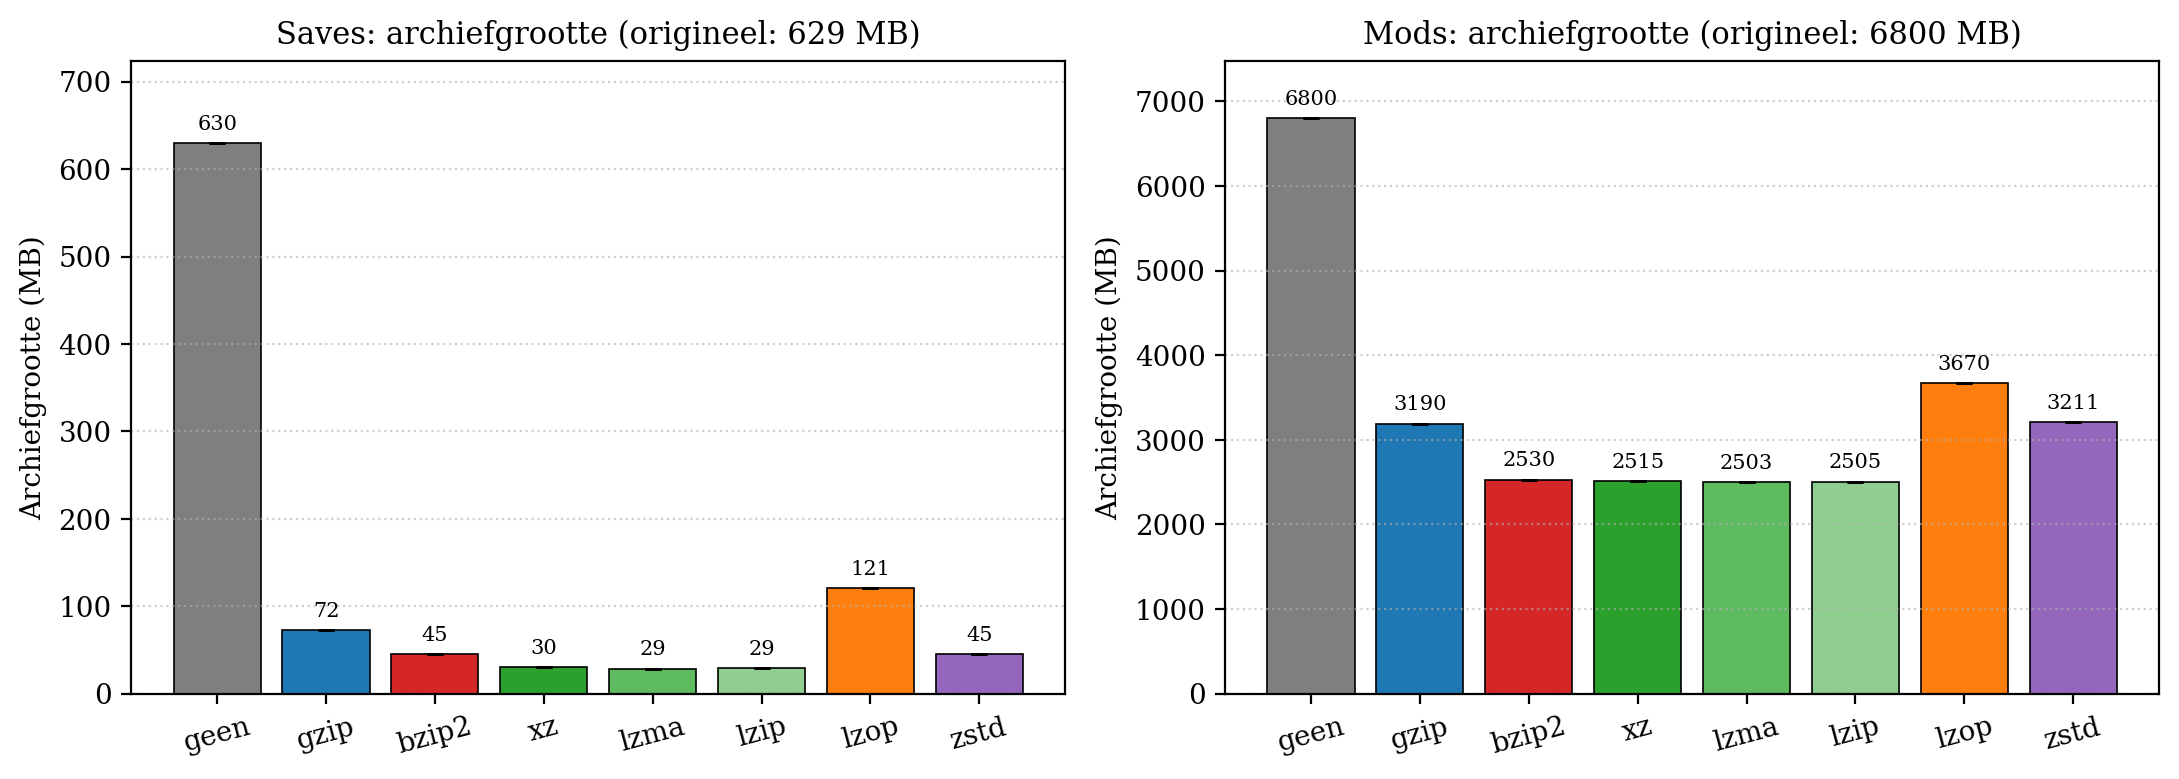
\includegraphics[width=\linewidth]{figures/fig_compression_size.png}
    \caption{Archiefgrootte per algoritme, voor de volledige back-up van respectievelijk de zes saves (links) en de drie mods (rechts). De ongecomprimeerde variant geldt als referentie.}
    \label{fig:compression-size}
\end{figure}

\paragraph{Saves.}
De zes savegames samen ($\sim$629~MB origineel) laten zich extreem goed comprimeren. \texttt{gzip} reduceert het archief tot $\sim$72~MB (ratio 0{,}115); de LZMA-familie haalt nog meer winst en duwt de archiefgrootte tot onder de 30~MB (ratio $\sim$0{,}046 -- 0{,}048). De spreiding tussen \texttt{xz}, \texttt{lzma} en \texttt{lzip} is verwaarloosbaar, ze gebruiken intern hetzelfde algoritme. Aan de andere kant van het spectrum staat \texttt{lzop}, dat slechts tot $\sim$121~MB inkort (ratio 0{,}192). \texttt{zstd} en \texttt{bzip2} landen beide rond $\sim$45~MB (ratio 0{,}072). Dat savegames zo sterk comprimeren wijst erop dat ze grotendeels uit gestructureerde tekstdata bestaan, met veel herhaling.

\paragraph{Mods.}
Bij de mods is het beeld dramatisch anders. Alle algoritmes convergeren rond een ratio van 0{,}37 -- 0{,}54, en het verschil tussen het beste algoritme (\texttt{lzma}, $\sim$2503~MB) en het slechtste (\texttt{lzop}, $\sim$3670~MB) is slechts een factor 1{,}5. \texttt{gzip}, \texttt{zstd} en \texttt{lzop} blijven steken rond $\sim$3200 -- 3670~MB. Voor de mod-werklast levert de keuze van het algoritme dus voornamelijk een afweging op tussen compressietijd en geheugengebruik, niet zozeer een verschil in eindgrootte.

\subsection{Compressie- en decompressietijd}
\label{subsec:compressie-tijd}

Figuur~\ref{fig:compression-time} toont de back-up- en restoretijd per algoritme. Wegens het zeer brede bereik wordt een logaritmische y-as gebruikt.

\begin{figure}[h]
    \centering
    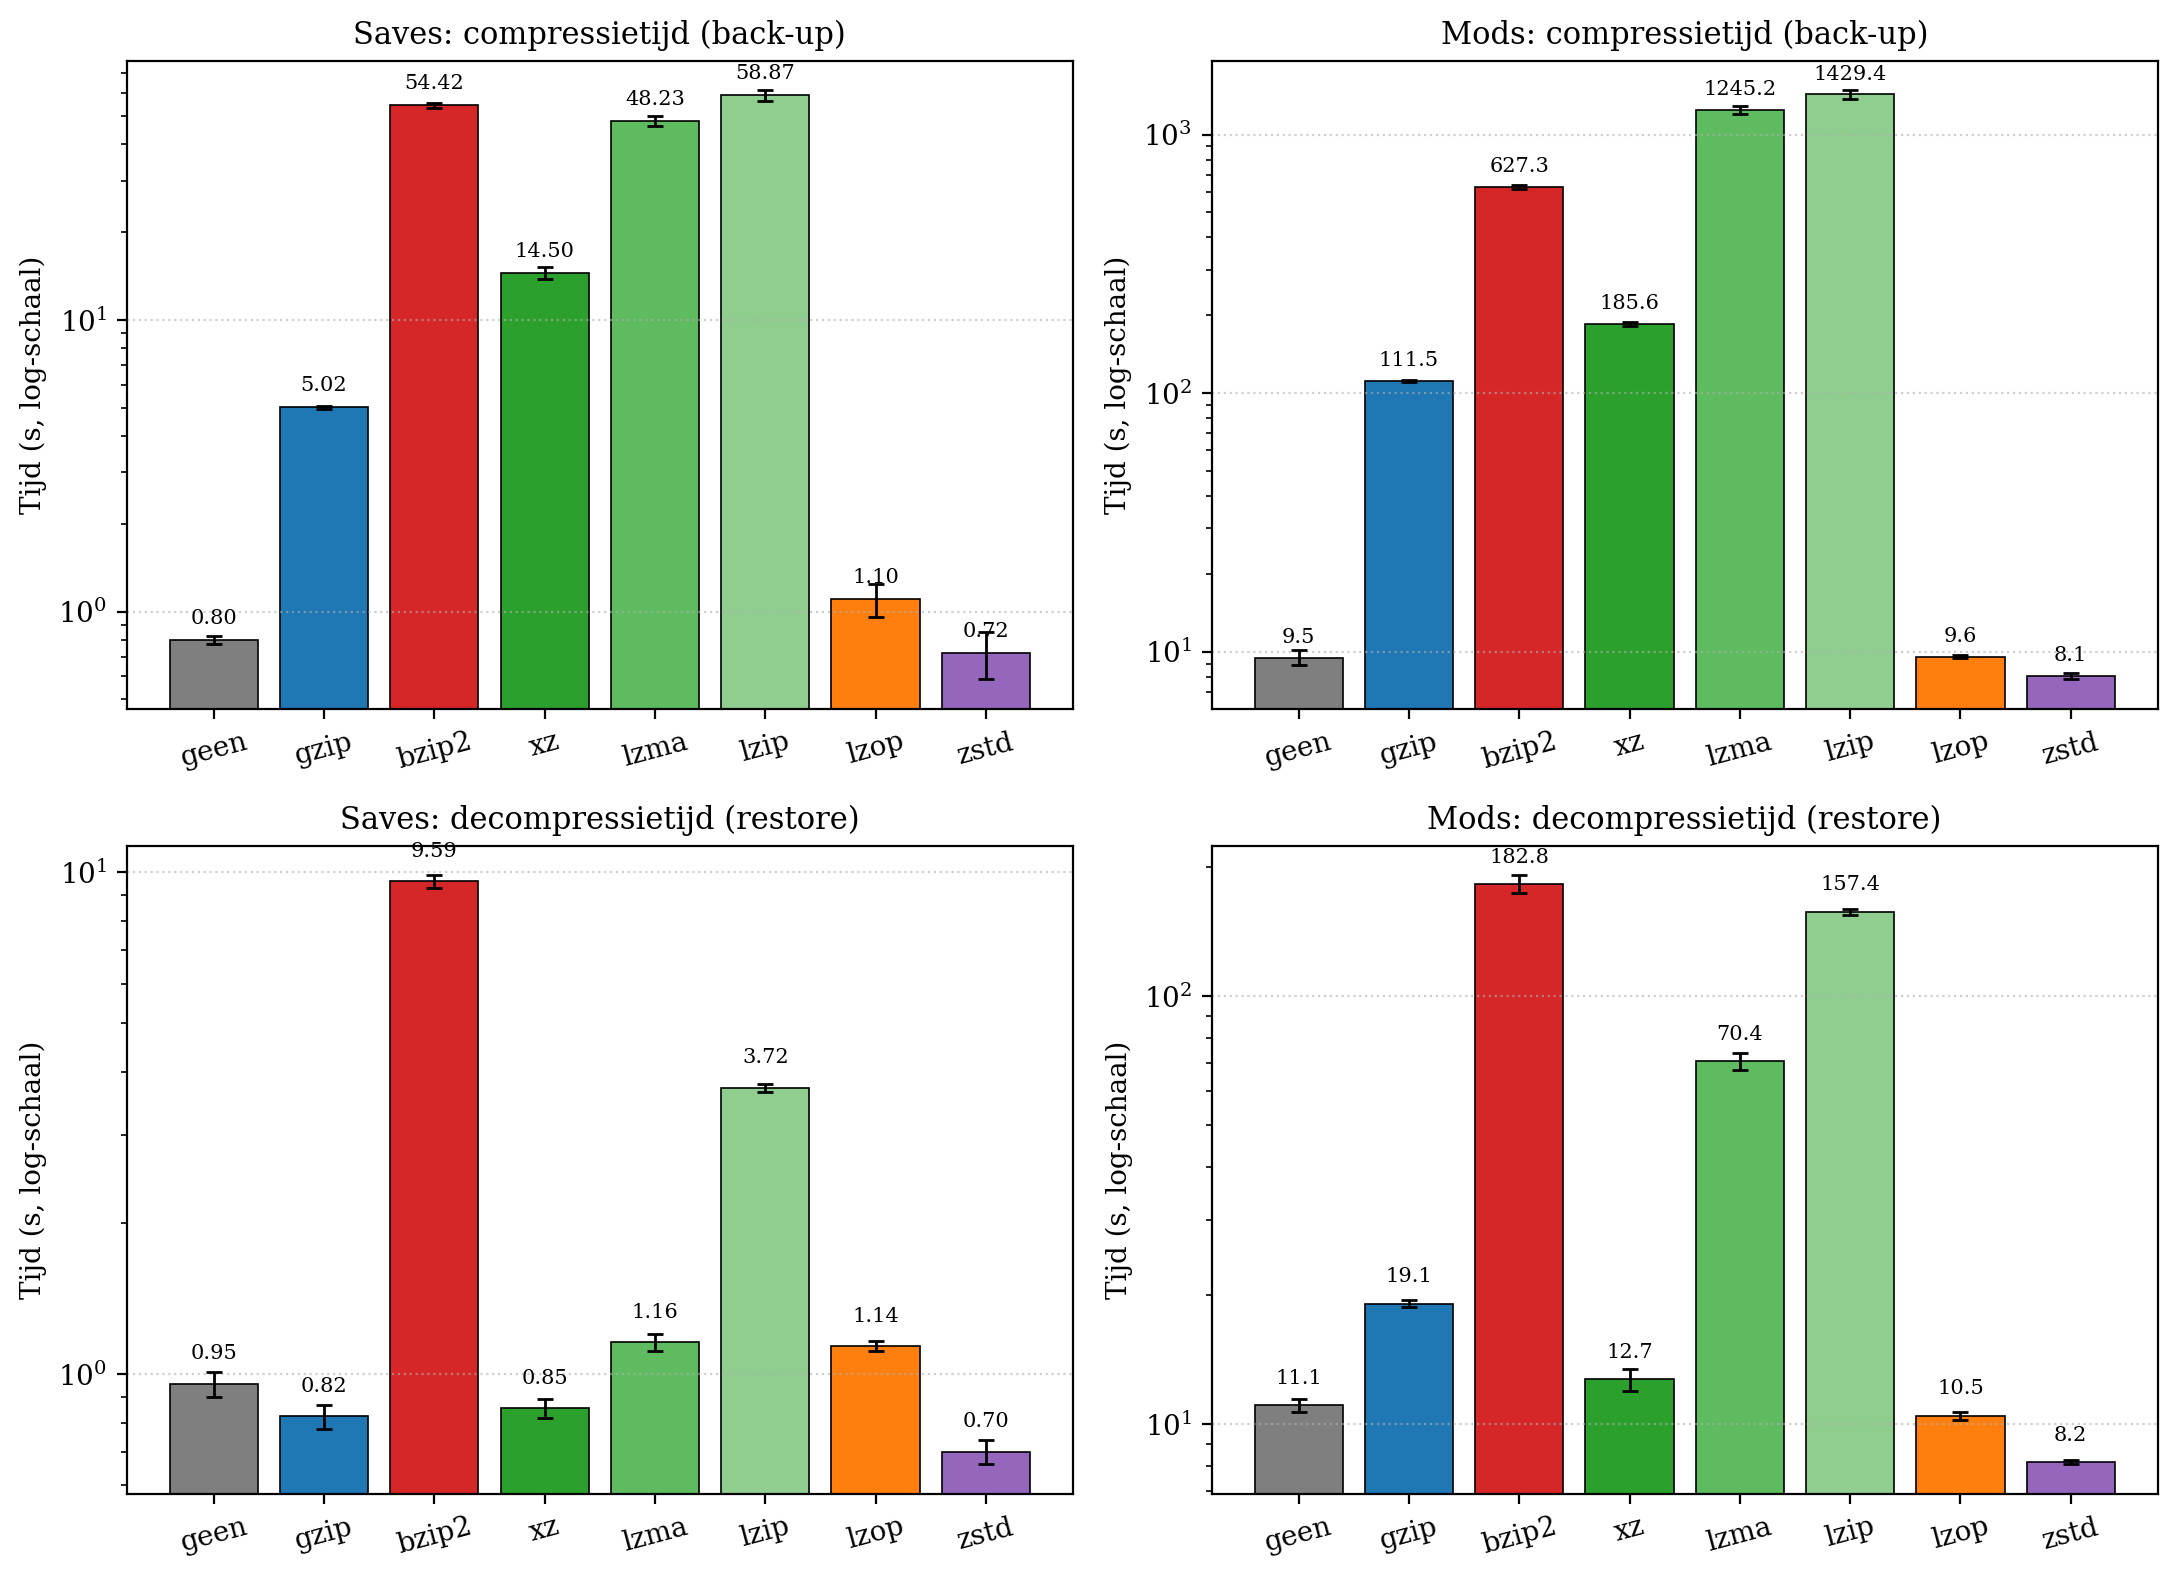
\includegraphics[width=\linewidth]{figures/fig_compression_time.png}
    \caption{Compressietijd (boven) en decompressietijd (onder) per algoritme, voor saves (links) en mods (rechts). De y-as is logaritmisch wegens het grote bereik. Foutbalken: standaardafwijking over 10 runs.}
    \label{fig:compression-time}
\end{figure}

\paragraph{Compressietijd (back-up).}
Voor de mods spreidt de compressietijd zich uit over drie orden van grootte: \texttt{zstd} en \texttt{lzop} blijven onder de 10 seconden, \texttt{gzip} doet er $\sim$112~s over, \texttt{xz} $\sim$186~s, \texttt{bzip2} $\sim$627~s, en \texttt{lzma}/\texttt{lzip} respectievelijk $\sim$1245~s en $\sim$1429~s. Dat een back-up van 6{,}5~GB met \texttt{lzip} bijna 24 minuten duurt, is voor een interactief back-upsysteem onaanvaardbaar. \texttt{zstd} is bovendien zelfs \emph{sneller} dan de ongecomprimeerde tar-back-up ($\sim$8{,}1~s tegenover $\sim$9{,}5~s). Dit is geen meetfout: \texttt{zstd} draait parallel over meerdere threads (zie sectie~\ref{subsec:compressie-cpu}) en compenseert de extra rekentijd door de I/O-belasting te verminderen, een gecomprimeerd archief is kleiner en hoeft minder bytes naar de SSD te schrijven.

Voor de saves geldt dezelfde rangorde, maar op een andere absolute schaal. \texttt{zstd} en \texttt{lzop} blijven onder 1{,}1~s, \texttt{gzip} doet er $\sim$5~s over, en de zware algoritmes (\texttt{bzip2}, \texttt{lzma}, \texttt{lzip}) zitten bij 48 -- 59~s. \texttt{xz} valt op met $\sim$14{,}5~s; opnieuw te verklaren door multithreading.

\paragraph{Decompressietijd (restore).}
Het beeld bij decompressie is fundamenteel anders. \texttt{zstd} ($\sim$8{,}2~s op mods, $\sim$0{,}70~s op saves) en \texttt{xz} zijn de snelste decompressors. \texttt{xz} ondersteunt namelijk parallelle decompressie, en presteert daarom drastisch beter dan zijn single-threaded familieleden \texttt{lzma} en \texttt{lzip}. \texttt{lzma} doet er $\sim$70~s over op de mods (factor 5{,}5 trager dan xz); \texttt{lzip} zelfs $\sim$157~s. \texttt{bzip2} is bij decompressie nog trager dan bij compressie ten opzichte van de LZMA-familie. Waar gzip en zstd typisch veel sneller decomprimeren dan comprimeren, blijft de decompressie van bzip2 relatief duur ($\sim$183~s op de mods). \texttt{lzop} is consistent snel maar wint hier geen significant voordeel ten opzichte van \texttt{zstd} of \texttt{xz}.

Voor een back-upsysteem dat in een rollbackscenario gebruikt zal worden, is de decompressietijd een zeer belangrijke factor. \texttt{lzip} en \texttt{bzip2} sluiten zichzelf hiermee effectief uit voor grote datasets: een restoreoperatie van enkele minuten op een mod-update van enkele gigabytes vraagt een extreem lange wachttijd op het kritieke moment waarop de gebruiker juist snel wil terugkeren.

\subsection{CPU-gebruik}
\label{subsec:compressie-cpu}

Figuur~\ref{fig:compression-cpu} toont het CPU-gebruik tijdens compressie en decompressie.

\begin{figure}[h]
    \centering
    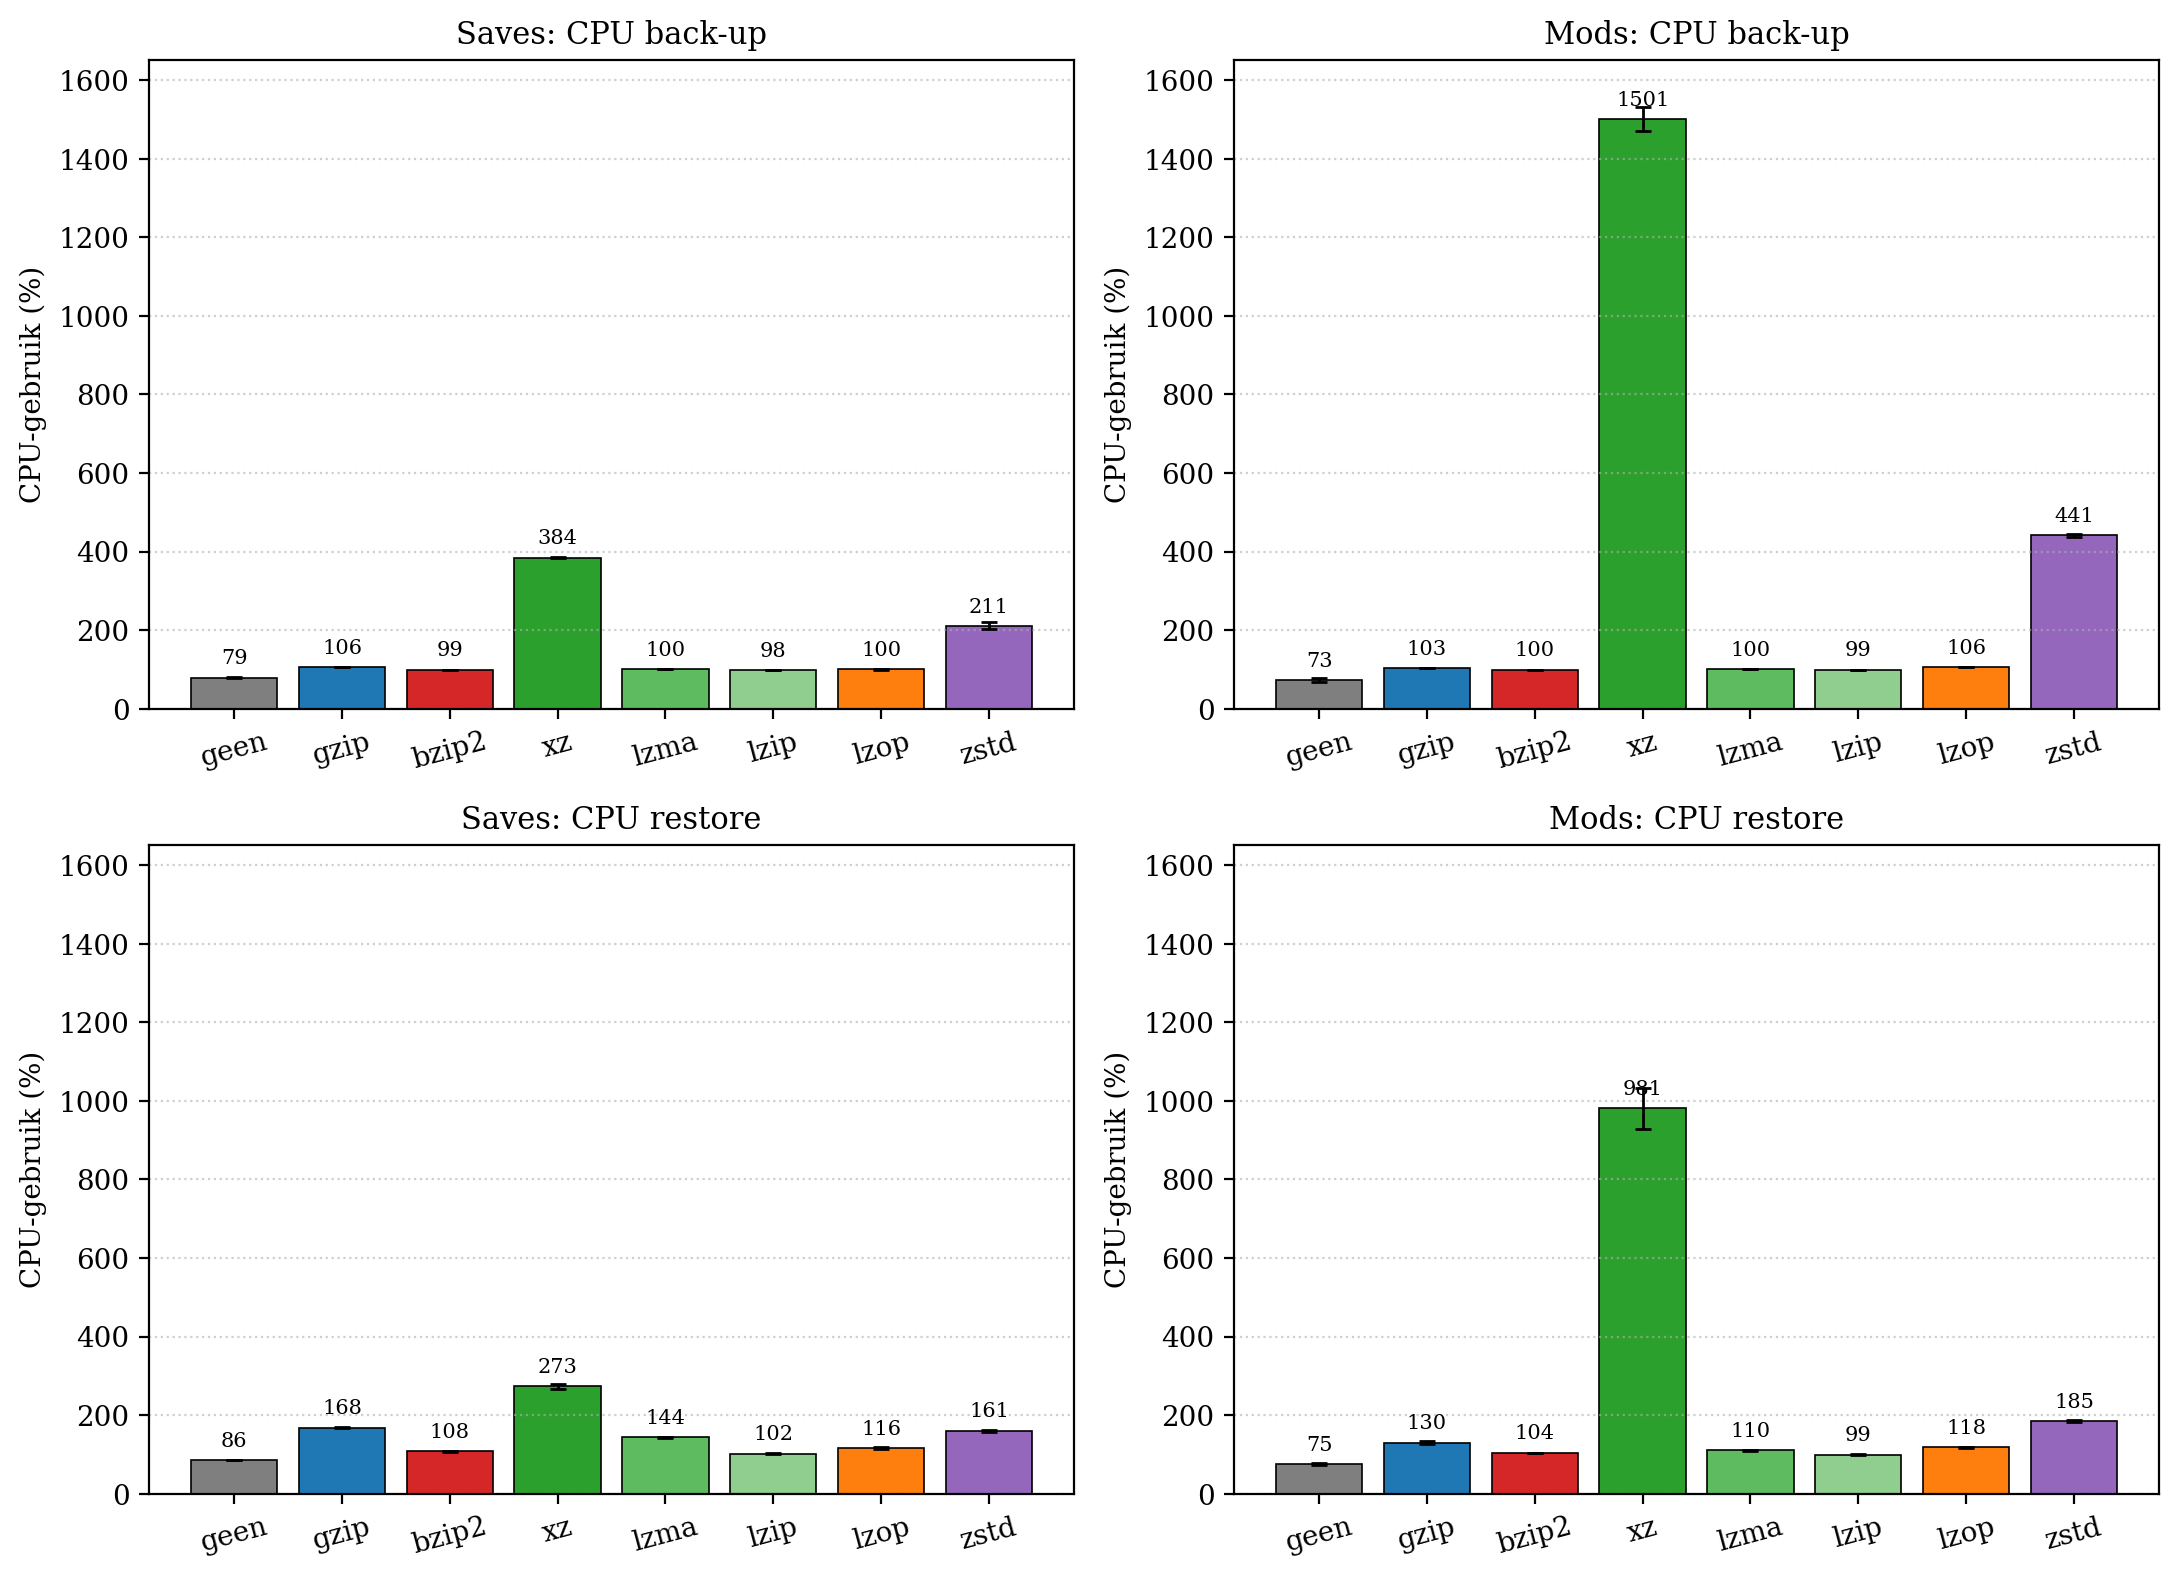
\includegraphics[width=\linewidth]{figures/fig_compression_cpu.png}
    \caption{CPU-gebruik per algoritme. De y-as is voor alle vier de panelen gelijk. Een waarde van 100\% komt overeen met één volledige thread; het maximum op deze 16-thread-CPU is 1600\%.}
    \label{fig:compression-cpu}
\end{figure}

\paragraph{Single-threaded versus multi-threaded.}
Het meest opvallende patroon is de scheiding tussen single-threaded algoritmes (\texttt{gzip}, \texttt{bzip2}, \texttt{lzma}, \texttt{lzip}, \texttt{lzop}: telkens rond 100\%) en multi-threaded algoritmes (\texttt{xz}, \texttt{zstd}). Op de mods bereikt \texttt{xz} $\sim$1500\% -- bijna 15 threads vol -- en \texttt{zstd} $\sim$441\% ($\sim$4 -- 5 threads). Dit verklaart waarom deze twee algoritmes ondanks hun rekenintensiteit nog vlotte wandkloktijden halen.

Op de saves is het multithreading-voordeel beperkter omdat de afzonderlijke archieven (gemiddeld $\sim$100~MB) te klein zijn om de parallelle pipeline van \texttt{xz} volledig te benutten: de gemeten waarde zakt naar $\sim$385\%. Ook \texttt{zstd} schakelt op kleine inputs minder threads in.

\paragraph{Decompressie.}
Bij decompressie zijn dezelfde patronen zichtbaar. \texttt{xz} blijft de enige van de LZMA-familie die multithreaded decomprimeert. Bij \texttt{lzma} en \texttt{lzip} blijft het CPU-gebruik beperkt tot $\sim$100\%. \texttt{zstd} bereikt $\sim$185\% bij decompressie van de mods, wat overeenkomt met ongeveer twee threads. \texttt{gzip} gebruikt bij decompressie meer dan 100\% (130 -- 168\%). Dit komt doordat de \texttt{tar}-pipeline de uitpak-thread parallel laat lopen met de schrijf-thread.

\subsection{Geheugengebruik}
\label{subsec:compressie-mem}

Figuur~\ref{fig:compression-mem} toont het piek-RSS per algoritme. De y-as is logaritmisch wegens het zeer grote bereik.

\begin{figure}[h]
    \centering
    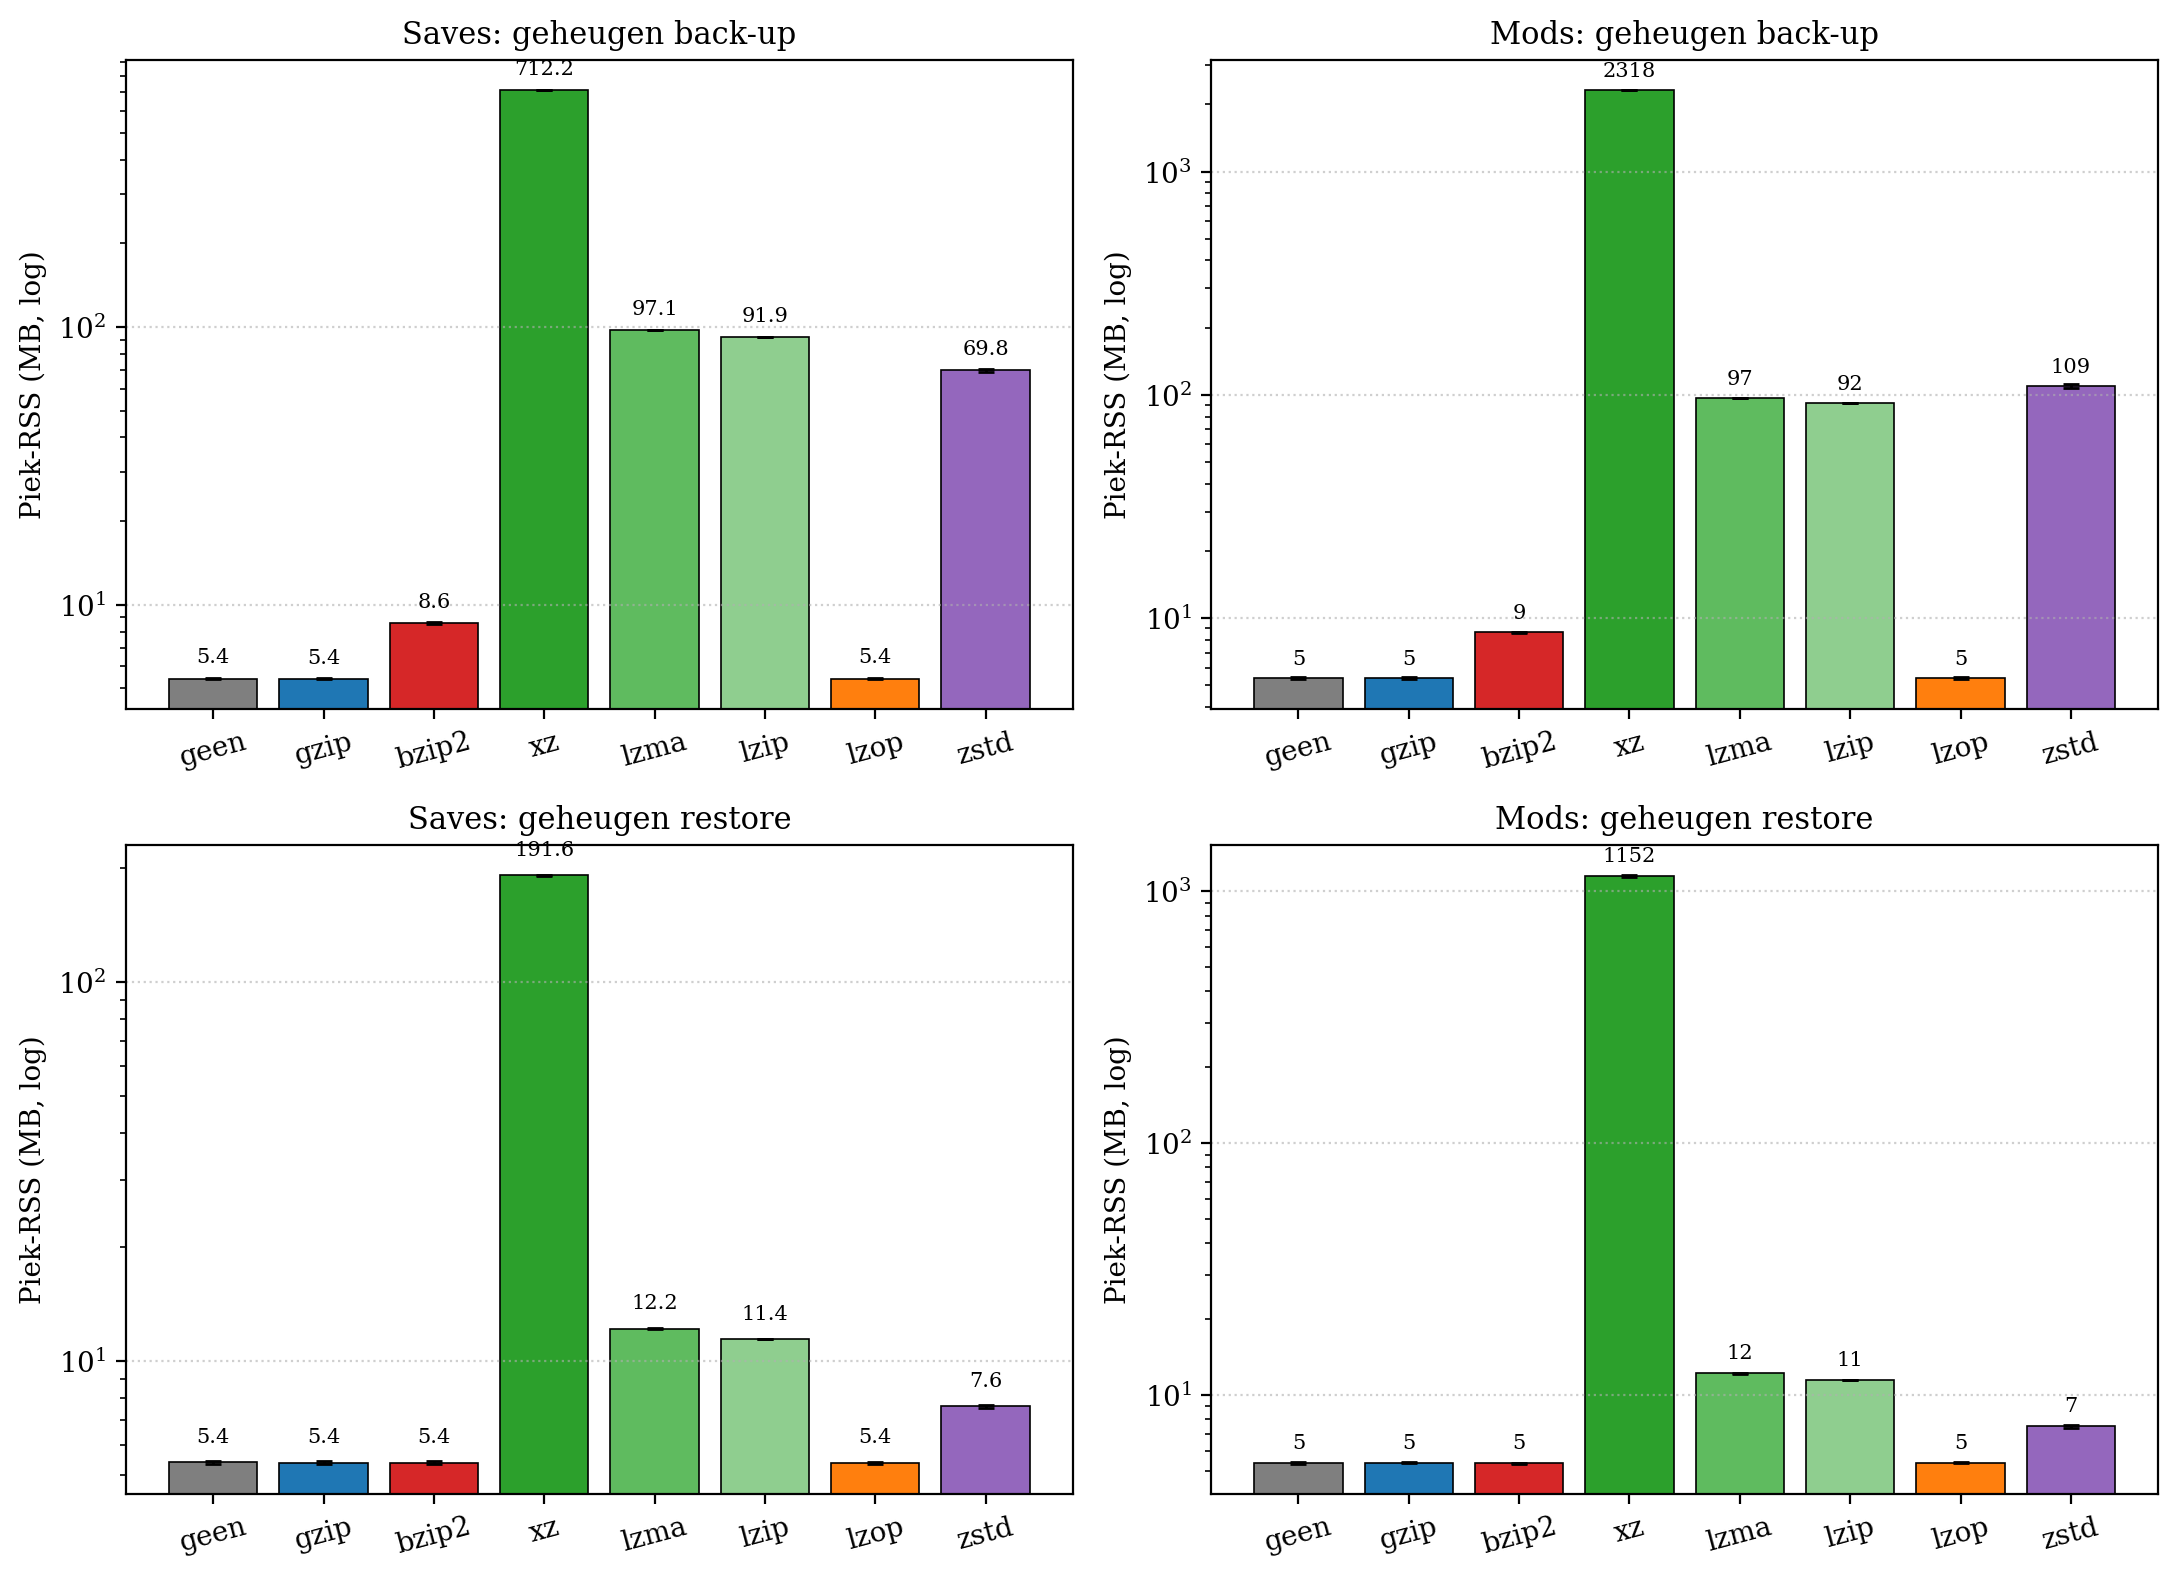
\includegraphics[width=\linewidth]{figures/fig_compression_mem.png}
    \caption{Piekgeheugengebruik per algoritme tijdens compressie (boven) en decompressie (onder). Y-as logaritmisch. De waarden zijn de hoogste piek over de hele dataset (alle saves of alle mods van één run).}
    \label{fig:compression-mem}
\end{figure}

\paragraph{Geheugen tijdens compressie.}
Het verschil tussen algoritmes is meer dan twee orden van grootte groot. \texttt{gzip} en \texttt{lzop} blijven beperkt tot $\sim$5~MB, identiek aan de ongecomprimeerde tar. \texttt{bzip2} gebruikt $\sim$9~MB, conform zijn vaste blokgrootte van 900~kB en zijn BWT-werkruimte. De LZMA-familie ligt rond $\sim$92 -- 97~MB (\texttt{lzma}, \texttt{lzip}) door het standaard woordenboek-formaat. \texttt{zstd} gebruikt $\sim$70 -- 110~MB. \texttt{xz} springt eruit met $\sim$712~MB op de saves en $\sim$2{,}3~GB op de mods. Dit enorm geheugengebruik is het gevolg van de combinatie van LZMA's groot woordenboek en de multithreading-strategie van \texttt{xz}, die per thread een eigen woordenboek bijhoudt.

\paragraph{Geheugen tijdens decompressie.}
Bij decompressie zakt het geheugengebruik aanzienlijk. Alle algoritmes behalve \texttt{xz} blijven onder 15~MB. \texttt{xz} gebruikt echter nog steeds $\sim$192~MB op saves en $\sim$1{,}15~GB op mods, omdat het voor parallelle decompressie eveneens meerdere woordenboeken in geheugen houdt. Single-threaded varianten \texttt{lzma} en \texttt{lzip} hebben slechts één woordenboek nodig en blijven daardoor onder de 13~MB. \texttt{bzip2} behoudt zijn kleine voetafdruk dankzij de blok-georiënteerde architectuur.

\subsection{Pareto-frontier: tijd versus archiefgrootte}
\label{subsec:pareto}

Een tweedimensionale afweging maakt de optimale keuzes veel gemakkelijker zichtbaar. Figuren~\ref{fig:pareto-backup} en~\ref{fig:pareto-restore} tonen elk algoritme als een punt in een ruimte met enerzijds tijd (logaritmisch) en anderzijds archiefgrootte. Algoritmes die op de Pareto-frontier liggen, zijn algoritmes waarvoor geen ander algoritme in deze test tegelijk sneller én kleiner is. Algoritmes die niet op de frontier liggen, zijn gedomineerd: er bestaat ten minste één alternatief dat in beide dimensies beter scoort.

\begin{figure}[h]
    \centering
    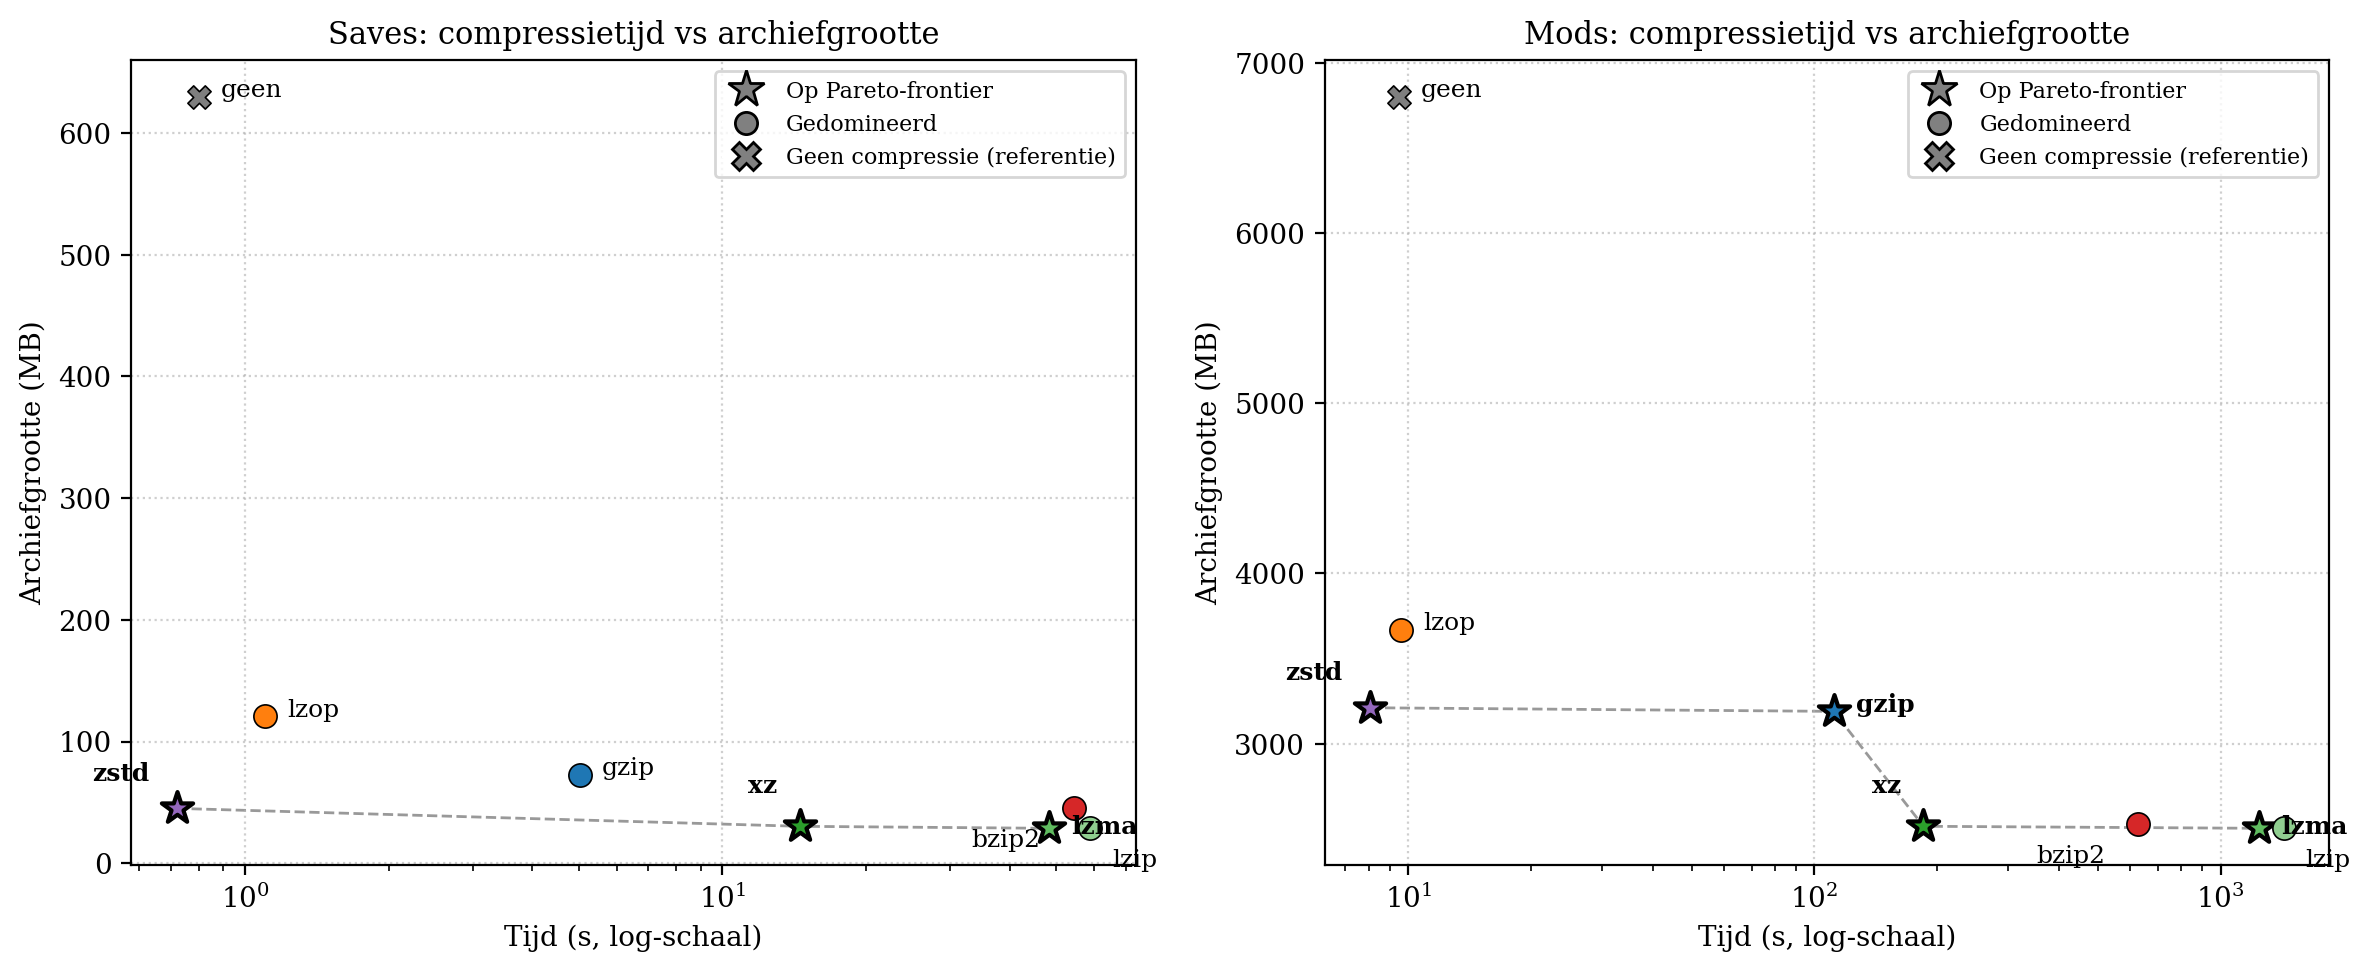
\includegraphics[width=\linewidth]{figures/fig_compression_pareto_backup.png}
    \caption{Pareto-frontier voor de back-upfase: compressietijd (x-as,
        log) tegenover archiefgrootte (y-as). Sterren markeren algoritmes op de Pareto-frontier; cirkels markeren gedomineerde algoritmes. Het kruis (geen compressie) wordt enkel getoond als referentie en werd uitgesloten uit de frontierberekening.}
    \label{fig:pareto-backup}
\end{figure}

\begin{figure}[h]
    \centering
    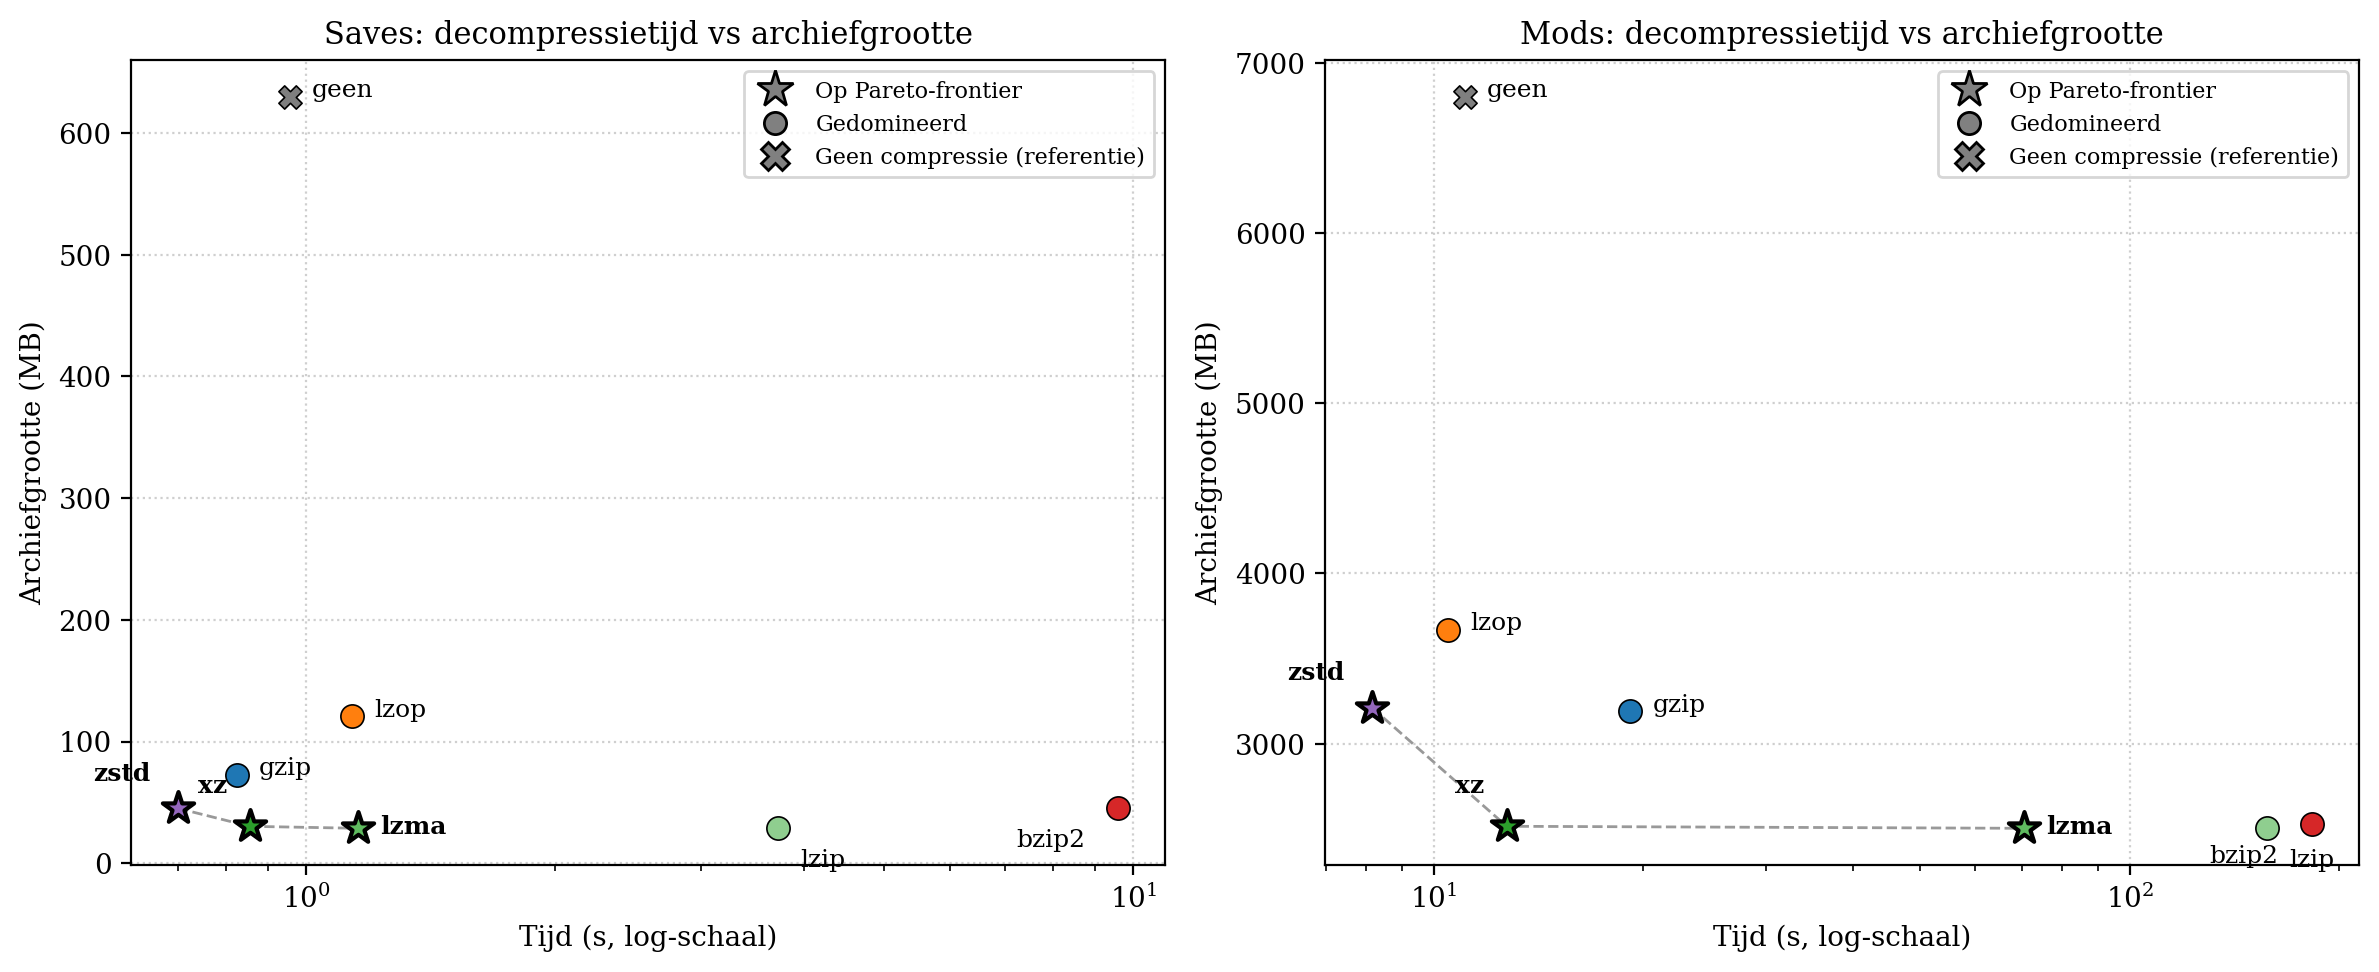
\includegraphics[width=\linewidth]{figures/fig_compression_pareto_restore.png}
    \caption{Pareto-frontier voor de restorefase: decompressietijd (x-as, log) tegenover archiefgrootte (y-as). Zelfde notatie als figuur~\ref{fig:pareto-backup}.}
    \label{fig:pareto-restore}
\end{figure}

\paragraph{Pareto-frontier voor de back-upfase.}
Bij beide datasets bestaat de back-upfrontier uit drie tot vier algoritmes. Voor de saves: \texttt{zstd} (snel, redelijke ratio), \texttt{xz} (middelmatige tijd, goede ratio), en \texttt{lzma}/\texttt{lzip} (traag, beste ratio). Voor de mods: \texttt{zstd}, \texttt{gzip}, \texttt{xz} en \texttt{lzma}. \texttt{lzop} en \texttt{bzip2} liggen onder de frontier en zijn dus gedomineerd: \texttt{lzop} wordt gedomineerd door \texttt{zstd} (zstd is sneller én kleiner), en \texttt{bzip2} wordt gedomineerd door \texttt{xz}.

\paragraph{Pareto-frontier voor de restorefase.}
De restoregrafieken geven een eenvoudiger beeld. Bij de saves: \texttt{zstd}, \texttt{xz} en \texttt{lzma} domineren alle overige algoritmes. \texttt{bzip2} en \texttt{lzip} vallen ver weg omdat hun decompressie traag is voor een ratio die geen voordeel oplevert ten opzichte van \texttt{xz}/\texttt{lzma}. Bij de mods is de frontier nog beknopter: \texttt{zstd}, \texttt{xz} en \texttt{lzma}, met \texttt{xz} duidelijk dominant boven \texttt{lzma} (kleinere ratio en snellere decompressie). \texttt{lzip} blijft op de frontier qua compressieratio bij sommige varianten, maar zijn $\sim$157~s decompressietijd op de mods plaatst hem ver buiten de praktische zone.

\subsection{Synthese en aanbeveling per dataset}
\label{subsec:compressie-conclusie}

Tabel~\ref{tab:compressie-summary} vat de belangrijkste meetwaarden
samen.

\begin{table}[h]
    \centering
    \caption{Compressie-algoritmes vergeleken op de volledige
        back-upmethode (totaal over de hele dataset). Tijden in seconden,
        grootte in MB, geheugen in MB.}
    \label{tab:compressie-summary}
    \small
    \begin{tabular}{lrrrrrrrr}
        \toprule
        & \multicolumn{4}{c}{\textbf{Saves ($\sim$629~MB origineel)}}
        & \multicolumn{4}{c}{\textbf{Mods ($\sim$6800~MB origineel)}} \\
        \cmidrule(lr){2-5}\cmidrule(lr){6-9}
        \textbf{Algoritme} & Comp. & Decomp. & Grootte & Mem
        & Comp. & Decomp. & Grootte & Mem \\
        \midrule
        geen           &   0{,}80  &   0{,}96  &   630 &     5
        &   9{,}48  &  12{,}58  &  6800 &     5 \\
        gzip           &   5{,}02  &   0{,}82  &    72 &     5
        & 111{,}51  &  19{,}14  &  3190 &     5 \\
        bzip2          &  54{,}42  &   9{,}59  &    45 &     9
        & 627{,}27  & 182{,}83  &  2530 &     9 \\
        xz             &  14{,}50  &   0{,}85  &    30 &   712
        & 185{,}59  &  12{,}73  &  2515 &  2318 \\
        lzma           &  48{,}23  &   1{,}16  &    29 &    97
        & 1245{,}18 &  70{,}43  &  2503 &    97 \\
        lzip           &  58{,}87  &   3{,}72  &    29 &    92
        & 1429{,}39 & 157{,}38  &  2505 &    92 \\
        lzop           &   1{,}10  &   1{,}14  &   121 &     5
        &   9{,}58  &  10{,}48  &  3670 &     5 \\
        zstd           &   0{,}72  &   0{,}70  &    45 &    70
        &   8{,}06  &   8{,}15  &  3211 &   109 \\
        \bottomrule
    \end{tabular}
\end{table}

\paragraph{Aanbeveling voor savegames.}
Bij de savegames komt \texttt{zstd} naar voren als de meest evenwichtige keuze: het comprimeert in $\sim$0{,}7~s tot $\sim$45~MB en decomprimeert in $\sim$0{,}7~s, met een geheugenvoetafdruk van $\sim$70~MB. Wie de allerkleinste archieven wil, kan kiezen voor \texttt{xz}, dat de archieven verder verkleint tot $\sim$30~MB met quasi-instantane decompressie ($\sim$0{,}85~s). De prijs is een back-uptijd die ongeveer 20 keer langer is en een geheugenpiek van $\sim$712~MB. Voor de typische gebruiker is dit een onnodig zwaar. \texttt{lzop} biedt geen meetbaar voordeel ten opzichte van \texttt{zstd} en wordt daarom afgeraden. \texttt{bzip2}, \texttt{lzma} en \texttt{lzip} verdedigen hun bestaansrecht hier niet: ze zijn allemaal aanzienlijk trager voor een zeer klein of onbestaand opslagvoordeel ten opzichte van \texttt{xz} of \texttt{zstd}.

\paragraph{Aanbeveling voor grote mods.}
Bij de mods wordt de keuze sterk beperkt door het feit dat de ratio's onderling weinig verschillen (een factor 1{,}5 tussen het beste en het slechtste algoritme), terwijl de tijden meer dan twee orden van grootte verschillen. \texttt{zstd} springt er hier sterk uit: het comprimeert sneller dan tar zonder compressie ($\sim$8~s tegenover $\sim$9{,}5~s), produceert een archief van $\sim$3{,}21~GB (een opslagbesparing van 53\%) en decomprimeert in slechts $\sim$8{,}2~s. De totale back-up + restore-cyclus duurt met \texttt{zstd} ongeveer 16 seconden, tegenover meer dan 26 minuten voor \texttt{lzip}. Het geheugengebruik blijft beperkt tot $\sim$109~MB, ruim binnen de mogelijkheden van een gemiddeld systeem.

De LZMA-varianten leveren bij de mods slechts $\sim$22\% kleinere archieven dan \texttt{zstd}, ten koste van een 23-keer langere back-uptijd (xz) tot zelfs een 177-keer langere back-uptijd (lzip). Voor de grote mods, waar ratios laag liggen door reeds gecomprimeerde assets, is deze niet acceptabel. \texttt{xz} blijft een goede keuze als de prioriteit op een zo klein mogelijke archiefgrootte ligt en het geheugengebruik van $\sim$2{,}3~GB geen probleem vormt, maar voor de typische thuisgebruiker is \texttt{zstd} duidelijk de optimale keuze.

\paragraph{Algemene observaties.}
Een aantal vaststellingen gelden voor beide datasets:

\begin{itemize}
    \item \textbf{\texttt{zstd} is in vrijwel alle dimensies de beste keuze.} Het haalt een goede compressieratio, comprimeert sneller dan ongecomprimeerde tar (door multithreading en verminderde I/O), decomprimeert minstens even snel, en blijft binnen aanvaardbare geheugengrenzen. Voor een back-upsysteem in een modlauncher is dit veruit het beste algoritme.
    \item \textbf{\texttt{lzop} wordt gedomineerd door \texttt{zstd}.} Vroeger was \texttt{lzop} de standaardkeuze voor maximale snelheid. \texttt{zstd} is op moderne hardware in vrijwel elke dimensie beter (sneller, kleinere archieven, vergelijkbaar geheugen).
    \item \textbf{\texttt{bzip2} en \texttt{lzip} zijn obsoleet voor deze werklast.} Hun trage decompressie (vooral voor \texttt{lzip}) maakt ze ongeschikt voor een rollbackscenario, terwijl ze geen compressievoordeel bieden ten opzichte van \texttt{xz} of \texttt{lzma}.
    \item \textbf{\texttt{xz} is een verdedigbare keuze voor maximaal kleine archieven}, mits het geheugengebruik geen probleem vormt. Voor mods is dit een aandachtspunt: een piek van $\sim$2{,}3~GB tijdens een back-up kan op een gamingsysteem merkbare impact hebben.
    \item \textbf{Grote mods comprimeren slecht door reeds gecomprimeerde assets.} De keuze van een agressief algoritme levert hier niet de winst op die ze bij saves geeft. Het is dus geen slecht idee om per datatype te differentiëren: voor saves kan een agressiever algoritme zinvol zijn, voor mods is een snel algoritme zoals \texttt{zstd} duidelijk de beste optie.
\end{itemize}


\section{Algemene ontwerprichtlijnen}
\label{sec:ontwerprichtlijnen}

In deze afsluitende sectie worden de bevindingen uit de analyse van de back-upmethodes (sectie~\ref{sec:synthese}) en de analyse van de compressie-algoritmes (sectie~\ref{subsec:compressie-conclusie}) samengebracht tot één set van ontwerprichtlijnen voor een back-up\-systeem in een modlauncher. De richtlijnen worden gegroepeerd rond drie thema's: de keuze van de back-upmethode, de keuze van het compressie-algoritme, en algemene architecturele principes.

\subsection{Richtlijnen voor de keuze van back-upmethode}

\begin{enumerate}
    \item \textbf{Snapshotting heeft de voorkeur wanneer het bestandssysteem dit toelaat.} Een copy-on-write snapshot-mechanisme (zoals btrfs of zfs) levert in alle geteste dimensies de beste resultaten: voorspelbare en lage back-up\-kost per back-uppunt, quasi-instantane rollbacks (in de orde van tientallen milliseconden), lage fysieke opslagvoetafdruk dankzij blok\-niveau-deduplicatie, en minimaal CPU- en geheugengebruik. Geen enkele andere geteste methode kan deze combinatie evenaren.
    \item \textbf{Wanneer snapshots niet beschikbaar zijn, is een incrementele methode het beste compromis.} De back-uptijd per punt is laag en het opslaggebruik is zuiniger dan dat van een volledige of differentiële strategie. De per-back-uppuntanalyse heeft echter aangetoond dat de cumulatieve restoretijd merkbaar oploopt naarmate er meer incrementen zijn. Een periodieke nieuwe basis-back-up is daarom wenselijk om de restoretijd binnen bruikbare grenzen te houden.
    \item \textbf{Een differentiële strategie wordt afgeraden.} De analyse heeft aangetoond dat differentieel geen meetbaar voordeel oplevert ten opzichte van incrementeel: de archieven groeien cumulatief met elke nieuwe back-up, het opslaggebruik ligt hoger, de back-uptijd is langer, en de restoretijd is nauwelijks beter dan bij incrementeel.
    \item \textbf{Een volledige back-up zonder bijkomende logica is zelden zinvol.} Voor de werklast van een modlauncher levert deze methode geen voordeel op. De methode is enkel verdedigbaar voor scenario's waar de dataset uitzonderlijk klein en eenmalig is.
\end{enumerate}

\subsection{Richtlijnen voor de keuze van compressie-algoritme}

\begin{enumerate}\setcounter{enumi}{4}
    \item \textbf{\texttt{zstd} is de standaardkeuze voor compressie.} Het algoritme laat op vrijwel geen enkele dimensie een steek vallen. Op de moddataset comprimeert het zelfs sneller dan een ongecomprimeerde tar-back-up, dankzij de combinatie van multithreading en de kleinere I/O-belasting van een gecomprimeerd archief. De compressieratio ligt voor saves bij $\sim$0{,}07 en voor mods bij $\sim$0{,}47, met een decompressietijd die in beide gevallen de snelste is van alle geteste algoritmes en een geheugengebruik die ruim binnen de mogelijkheden van een gamingsysteem blijft.
    \item \textbf{\texttt{xz} is de optionele keuze voor maximale opslagbesparing.} Voor gebruikers waarvoor archiefgrootte primair is en geheugengebruik geen probleem is, levert \texttt{xz} archieven op die nog $\sim$22\% kleiner zijn dan die van \texttt{zstd}.
    \item \textbf{De overige algoritmes worden afgeraden.} \texttt{lzop} wordt in alle dimensies gedomineerd door \texttt{zstd}. \texttt{gzip} levert geen voordeel ten opzichte van \texttt{zstd} en is bovendien single-threaded. \texttt{bzip2} en \texttt{lzip} hebben een trage decompressie die ze ongeschikt maakt voor een rollback- scenario. \texttt{lzma} is in essentie hetzelfde algoritme als \texttt{xz} maar zonder multithreading en is daardoor altijd trager.
    \item \textbf{Differentieer per datatype.} Saves comprimeren uitstekend (ratio $\sim$0{,}07 met \texttt{zstd}); mods bevatten reeds gecomprimeerde assets en leveren bij geen enkel algoritme een ratio onder $\sim$0{,}37 op. Een agressiever algoritme inzetten voor de mods levert dus weinig extra winst op, terwijl de tijdkost dramatisch toeneemt. Een back-upsysteem kan eventueel een ander algoritme inzetten naargelang het type data, maar in de praktijk is \texttt{zstd} voor beide gevallen een zeer goede optie.
\end{enumerate}

\subsection{Algemene architecturele principes}

\begin{enumerate}\setcounter{enumi}{8}
    \item \textbf{Het back-upsysteem moet lokaal functioneren.} Zoals besproken in sectie~\ref{subsec:geen-cloud} is een cloud-gebaseerde back-up niet geschikt voor de context van een modlauncher: het spel kan offline gespeeld worden en mods kunnen meerdere gigabytes groot zijn. De back-up moet dus kunnen plaatsvinden zonder afhankelijk te zijn van een netwerkverbinding. Een optionele synchronisatie naar een externe locatie kan worden toegevoegd, maar mag geen vereiste zijn voor de basisfunctionaliteit.
    \item \textbf{De combinatie van methode en compressie is grotendeels orthogonaal.} Voor opstellingen met btrfs blijft de snapshotmethode primair en is compressie niet van toepassing (btrfs ondersteunt zelf transparante compressie, wat een afzonderlijke optimalisatie is buiten het bereik van dit onderzoek). Voor opstellingen waarin tar wordt gebruikt, levert de combinatie \texttt{tar + zstd} (incrementeel) de beste algemene afweging op: \texttt{zstd} voegt zo weinig extra rekentijd toe dat de gunstige eigenschappen van de incrementele methode behouden blijven, terwijl de archiefgrootte significant afneemt.
    \item \textbf{Voorspelbaarheid is een ontwerp\-eigenschap.} De analyses tonen aan dat snapshot-back-ups quasi-constante kosten hebben per back-up, terwijl tar-gebaseerde methodes meer variabiliteit vertonen, vooral de volledige restore op grote archieven. Voor een back-upsysteem dat geautomatiseerd wordt (bijvoorbeeld bij elke mod-update), is voorspelbaarheid een belangrijke kwaliteit: de gebruiker mag niet geconfronteerd worden met onverwachte wachttijden die de spelervaring verstoort.
\end{enumerate}

\subsection{Samenvatting van de aanbevolen configuratie}

Op basis van het bovenstaande wordt de volgende standaardconfiguratie voor een modlauncher\-back\-up\-systeem aanbevolen:

\begin{itemize}
    \item \textbf{Primaire methode:} btrfs-snapshots, indien het bestandssysteem dit ondersteunt. Snapshots bij elke savegame en bij elke mod-installatie of -update.
    \item \textbf{Secundaire methode:} incrementele \texttt{tar}- back-ups gecomprimeerd met \texttt{zstd}, met periodiek een nieuwe basis-back-up om de restoretijd onder controle te houden.
    \item \textbf{Locatie:} lokaal, met een optionele synchronisatiemodule naar externe opslag voor wie dat wenst.
\end{itemize}
